%!TEX program = xelatex
% 完整编译: xelatex -> biber/bibtex -> xelatex -> xelatex
\documentclass[lang=cn,11pt,a4paper]{elegantpaper}

\title{实验报告}
\author{Wenchong Huang}
\date{\zhtoday}


% 本文档命令
\usepackage{array, float}
\newcommand{\ccr}[1]{\makecell{{\color{#1}\rule{1cm}{1cm}}}}

\begin{document}

\maketitle

\section{规则边界}

在这一节中,我们求解规则边界$\Omega=(0,1)^2$中的Poisson方程。

\subsection{Dirichlet条件}

考虑由精确解$u_1(x,y)=e^{\sin x+y}$导出的Dirichlet边值问题
\begin{equation}
  \left\{
    \begin{array}{l}
      -\Delta u = -(1-\sin x+\cos^2 x)e^{\sin x + y},\quad x\in\Omega \\
      u|_{\partial \Omega}=e^{\sin x + y}
    \end{array}
  \right. .
\end{equation}

用$n=16,32,64,128$的网格求解,所得数值解如下图。

\begin{figure}[htbp]
  \centering
  \begin{minipage}[t]{0.24\linewidth}
      \centering
      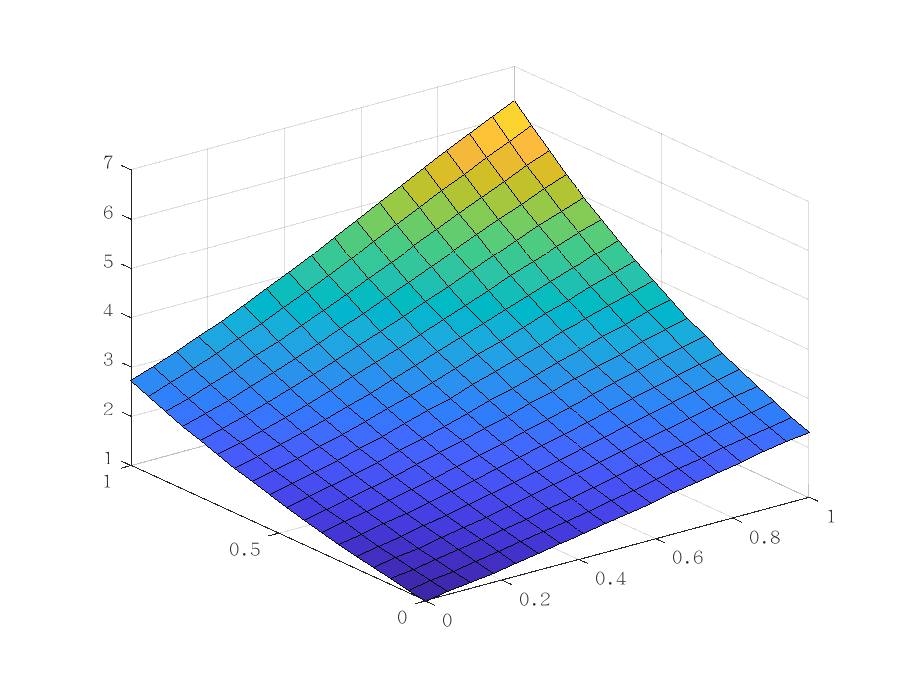
\includegraphics[width=0.95\linewidth]{figure/result_problem1_D_r_n=16.eps}
      \caption*{$n=16$}
  \end{minipage}
  \begin{minipage}[t]{0.24\linewidth}
    \centering
    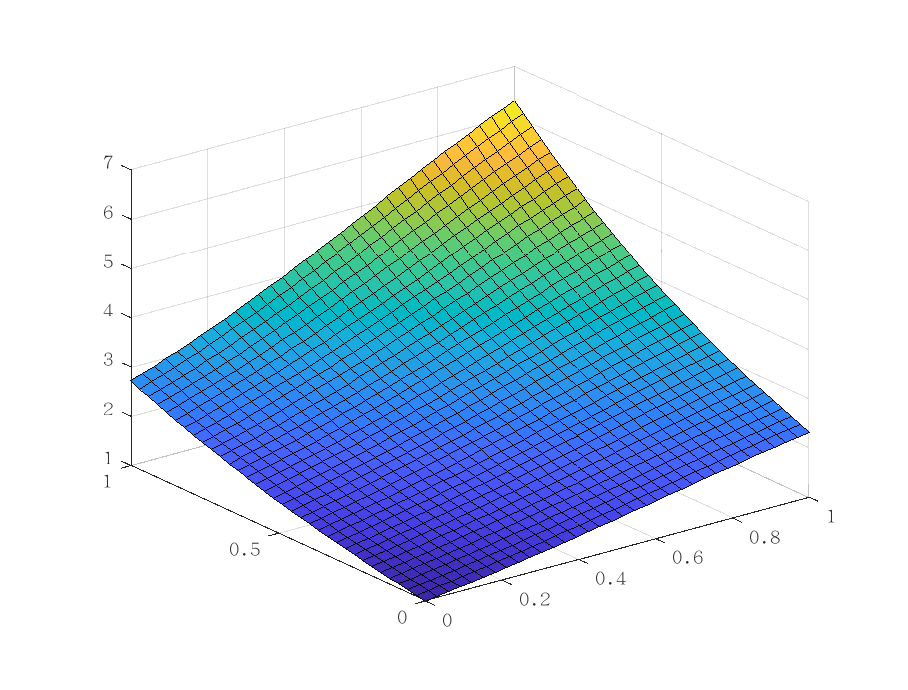
\includegraphics[width=0.95\linewidth]{figure/result_problem1_D_r_n=32.eps}
    \caption*{$n=32$}
  \end{minipage}
  \begin{minipage}[t]{0.24\linewidth}
    \centering
    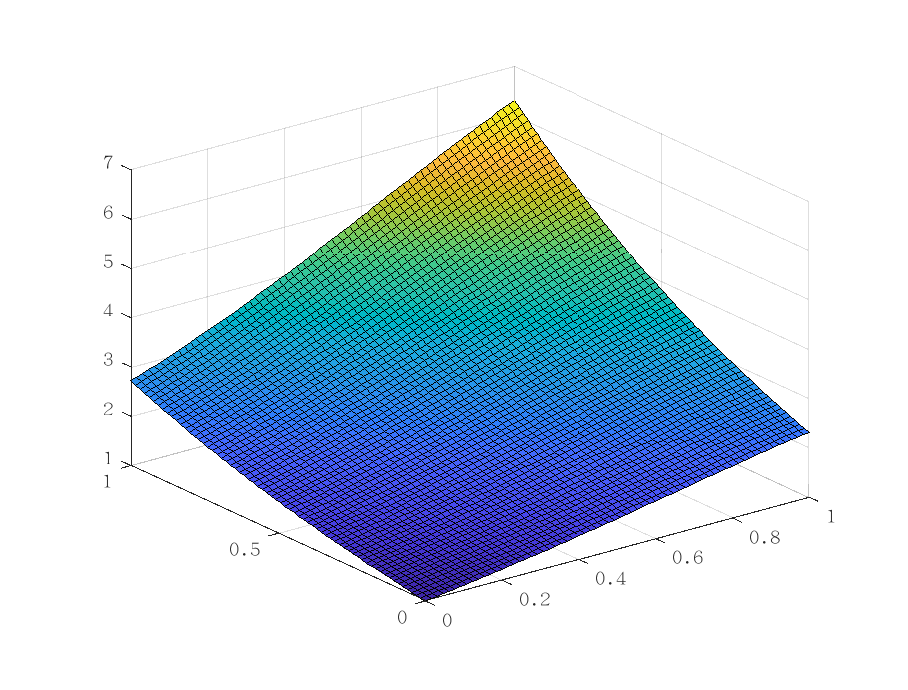
\includegraphics[width=0.95\linewidth]{figure/result_problem1_D_r_n=64.eps}
    \caption*{$n=64$}
  \end{minipage}
  \begin{minipage}[t]{0.24\linewidth}
    \centering
    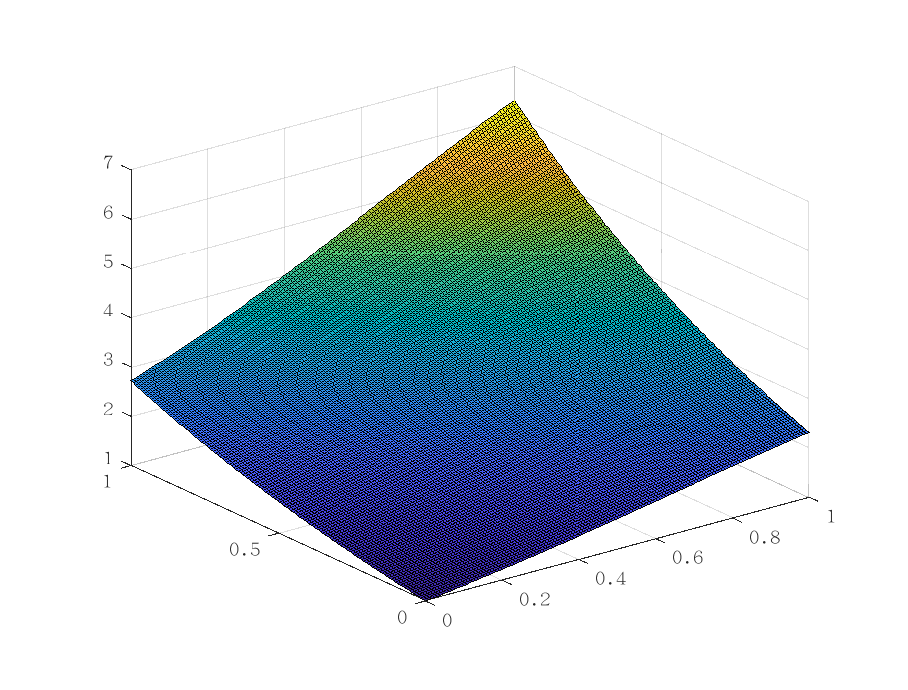
\includegraphics[width=0.95\linewidth]{figure/result_problem1_D_r_n=128.eps}
    \caption*{$n=128$}
  \end{minipage}
\end{figure}

与真实解作差,所得各点残差的图像如下。

\begin{figure}[htbp]
  \centering
  \begin{minipage}[t]{0.24\linewidth}
      \centering
      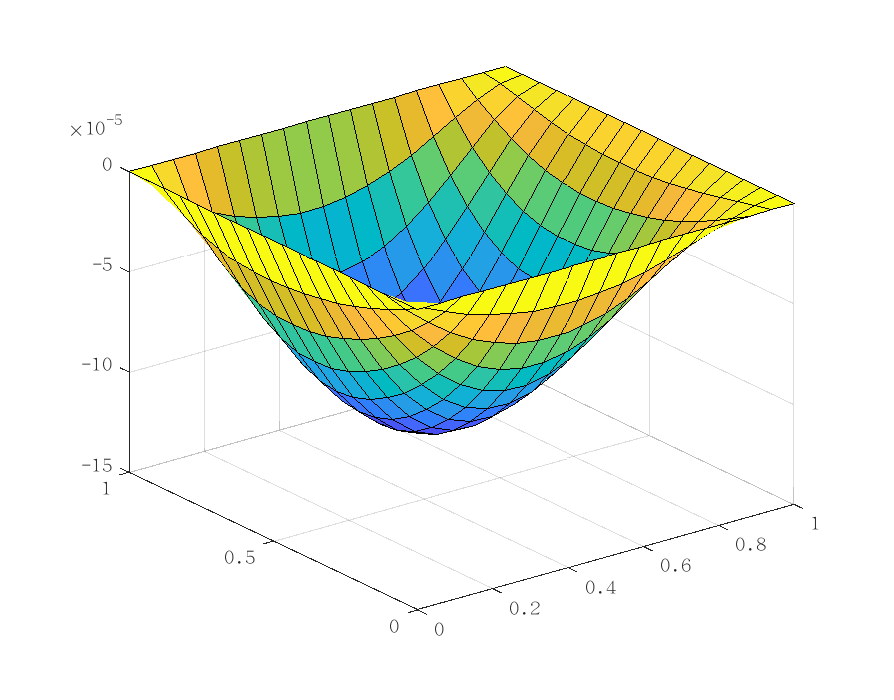
\includegraphics[width=0.95\linewidth]{figure/error_problem1_D_r_n=16.eps}
      \caption*{$n=16$}
  \end{minipage}
  \begin{minipage}[t]{0.24\linewidth}
    \centering
    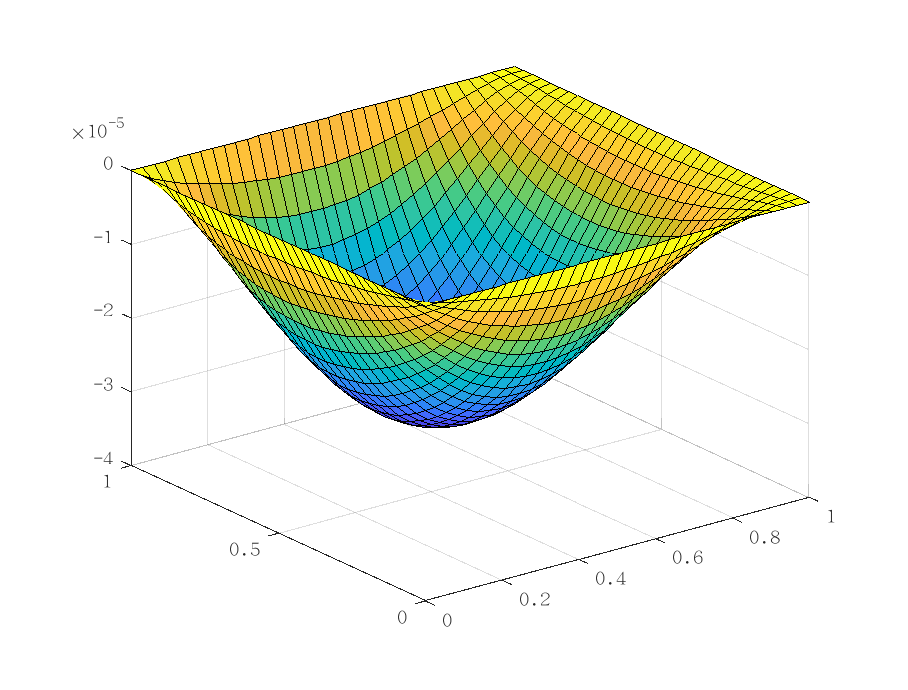
\includegraphics[width=0.95\linewidth]{figure/error_problem1_D_r_n=32.eps}
    \caption*{$n=32$}
  \end{minipage}
  \begin{minipage}[t]{0.24\linewidth}
    \centering
    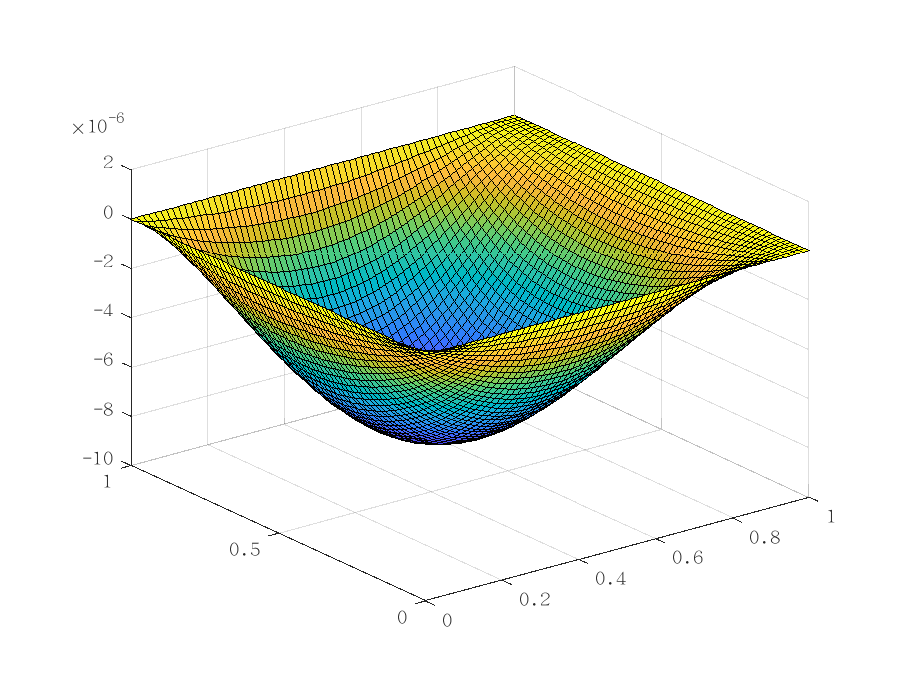
\includegraphics[width=0.95\linewidth]{figure/error_problem1_D_r_n=64.eps}
    \caption*{$n=64$}
  \end{minipage}
  \begin{minipage}[t]{0.24\linewidth}
    \centering
    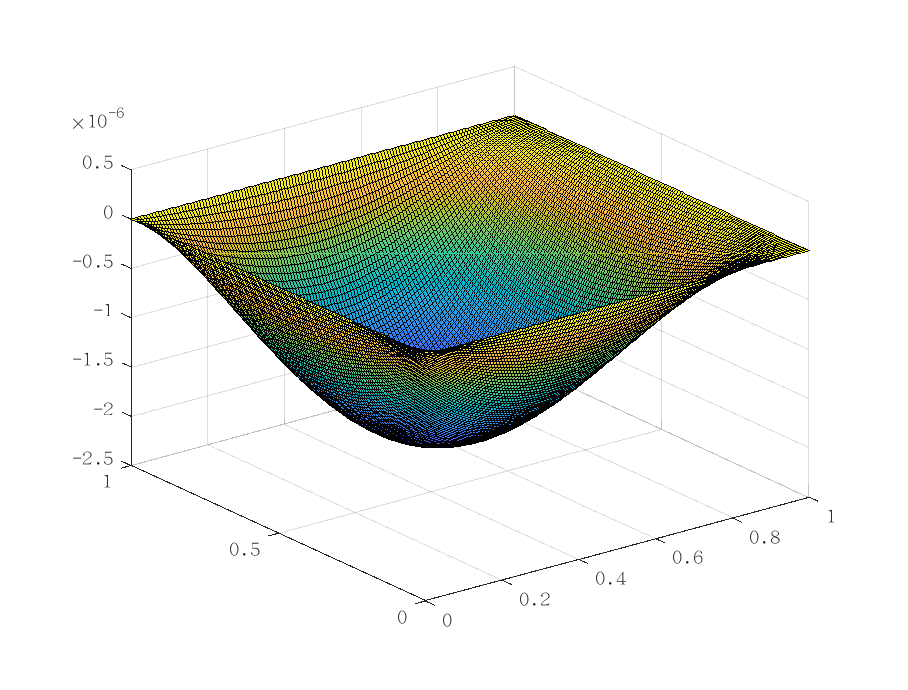
\includegraphics[width=0.95\linewidth]{figure/error_problem1_D_r_n=128.eps}
    \caption*{$n=128$}
  \end{minipage}
\end{figure}

可以看到,在Dirichlet条件下,格点越靠近边界,最终的计算误差越小。将数值解与真实解的误差用范数估计,并根据$n=64$增加到$n=128$时误差减小的倍数,估计各范数下的收敛率,结果如下表。

\begin{table}[H]
  \centering
  \begin{tabular}{c|cccc|c}
  \textbf{$n$}        & 16                   & 32                   & 64                   & 128                  & 收敛率 \\ \hline
  $1$-norm error      & $5.79\times 10^{-5}$ & $1.46\times 10^{-5}$ & $3.65\times 10^{-6}$ & $9.12\times 10^{-7}$ & $2.00$\\
  $2$-norm error      & $6.72\times 10^{-5}$ & $1.73\times 10^{-5}$ & $4.40\times 10^{-6}$ & $1.11\times 10^{-6}$ & $1.99$\\
  $\infty$-norm error & $1.22\times 10^{-4}$ & $3.24\times 10^{-5}$ & $8.36\times 10^{-6}$ & $2.12\times 10^{-6}$ & $1.98$
  \end{tabular}
\end{table}

再用函数
\begin{equation}
  u_2(x,y)=\log\left(10(x+y)^2+(x-y)^2+\frac{1}{2}\right)
\end{equation}

导出相应的Dirichlet边值问题,用数值方法求解,得到误差与收敛率如下表。

\begin{table}[H]
  \centering
  \begin{tabular}{c|cccc|c}
  \textbf{$n$}        & 16                   & 32                   & 64                   & 128                  & 收敛率 \\ \hline
  $1$-norm error      & $6.23\times 10^{-4}$ & $1.60\times 10^{-4}$ & $4.02\times 10^{-5}$ & $1.01\times 10^{-5}$ & $1.99$\\
  $2$-norm error      & $1.01\times 10^{-3}$ & $2.63\times 10^{-4}$ & $6.71\times 10^{-5}$ & $1.69\times 10^{-5}$ & $1.99$\\
  $\infty$-norm error & $4.05\times 10^{-3}$ & $1.08\times 10^{-3}$ & $2.77\times 10^{-4}$ & $7.06\times 10^{-5}$ & $1.97$
  \end{tabular}
\end{table}

再用函数
\begin{equation}
  u_3(x,y)=e^{\left( 10(x-0.5)^2+(y-0.5)^2 \right)}-1
\end{equation}

导出相应的Dirichlet边值问题,用数值方法求解,得到误差与收敛率如下表。

\begin{table}[H]
  \centering
  \begin{tabular}{c|cccc|c}
  \textbf{$n$}        & 16                   & 32                   & 64                   & 128                  & 收敛率 \\ \hline
  $1$-norm error      & $0.180$ & $4.69\times 10^{-2}$ & $1.19\times 10^{-2}$ & $2.98\times 10^{-3}$ & $2.00$\\
  $2$-norm error      & $0.189$ & $5.02\times 10^{-2}$ & $1.28\times 10^{-2}$ & $3.24\times 10^{-3}$ & $1.98$\\
  $\infty$-norm error & $0.262$ & $7.16\times 10^{-2}$ & $1.86\times 10^{-2}$ & $4.73\times 10^{-3}$ & $1.98$
  \end{tabular}
\end{table}

上述三个测试函数均符合2阶收敛的理论结果。

\subsection{Neumann条件}

考虑由精确解$u_1(x,y)=e^{\sin x+y}$导出的Neumann边值问题
\begin{equation}
  \left\{
    \begin{array}{l}
      -\Delta u = -(1-\sin x+\cos^2 x)e^{\sin x + y},\quad x\in\Omega, \\
      \frac{\partial u}{\partial \mathbf{n}}|_{x=0}=-e^{y},\\
      \frac{\partial u}{\partial \mathbf{n}}|_{x=1}=\cos 1 \cdot e^{\sin 1 + y},\\
      \frac{\partial u}{\partial \mathbf{n}}|_{y=0}=-e^{\sin x},\\
      \frac{\partial u}{\partial \mathbf{n}}|_{y=1}=e^{\sin x+1}
    \end{array}
  \right. .
\end{equation}

用$n=16,32,64,128$的网格求解,并与真实解作差。由于Neumann边值条件下,数值解与真实解会相差一个常数,在我们验证误差时,取格点上真实解减去数值解的最大最小值平均$C$,让数值解加上$C$后再作误差计算。所得各点残差的图像如下。

\begin{figure}[htbp]
  \centering
  \begin{minipage}[t]{0.24\linewidth}
      \centering
      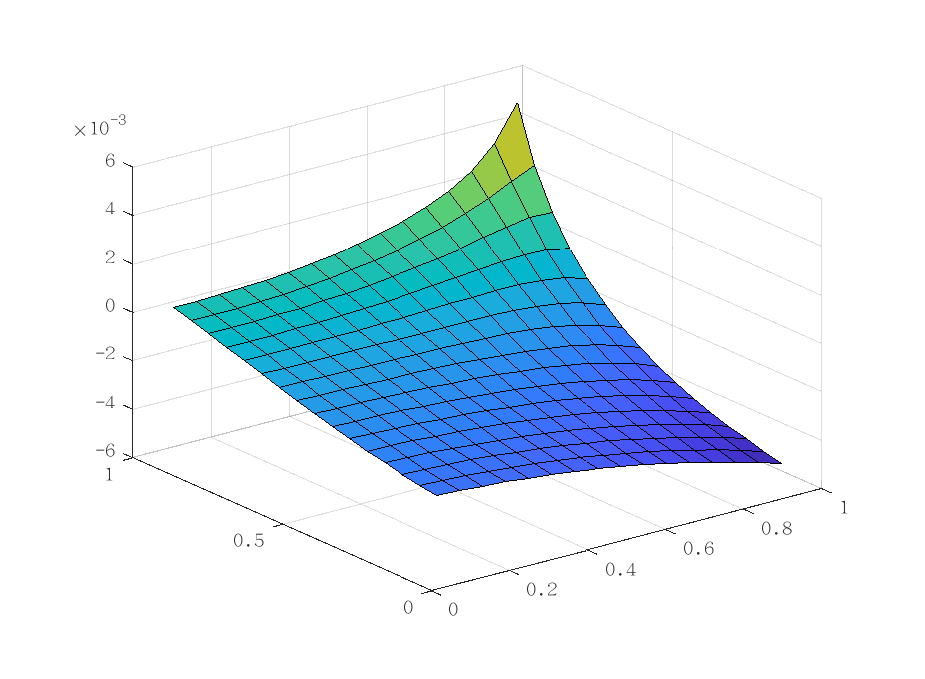
\includegraphics[width=0.95\linewidth]{figure/error_problem1_N_r_n=16.eps}
      \caption*{$n=16$}
  \end{minipage}
  \begin{minipage}[t]{0.24\linewidth}
    \centering
    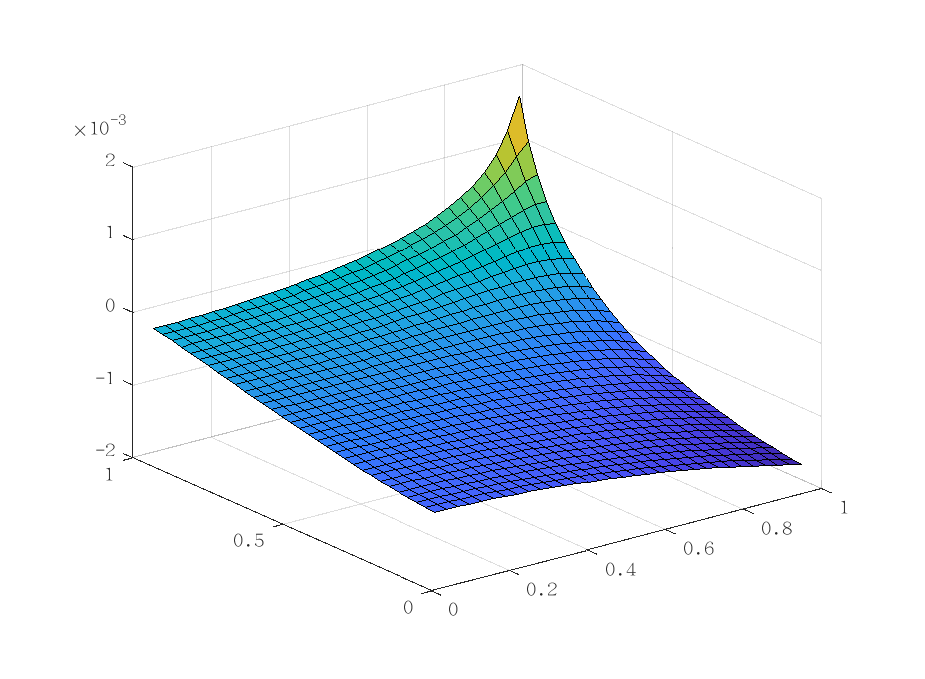
\includegraphics[width=0.95\linewidth]{figure/error_problem1_N_r_n=32.eps}
    \caption*{$n=32$}
  \end{minipage}
  \begin{minipage}[t]{0.24\linewidth}
    \centering
    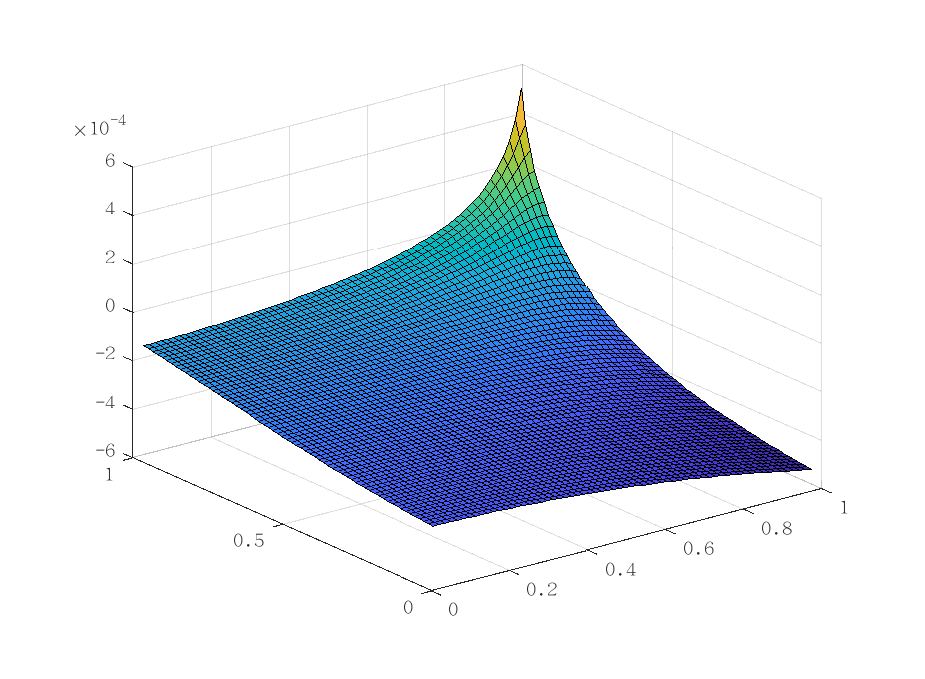
\includegraphics[width=0.95\linewidth]{figure/error_problem1_N_r_n=64.eps}
    \caption*{$n=64$}
  \end{minipage}
  \begin{minipage}[t]{0.24\linewidth}
    \centering
    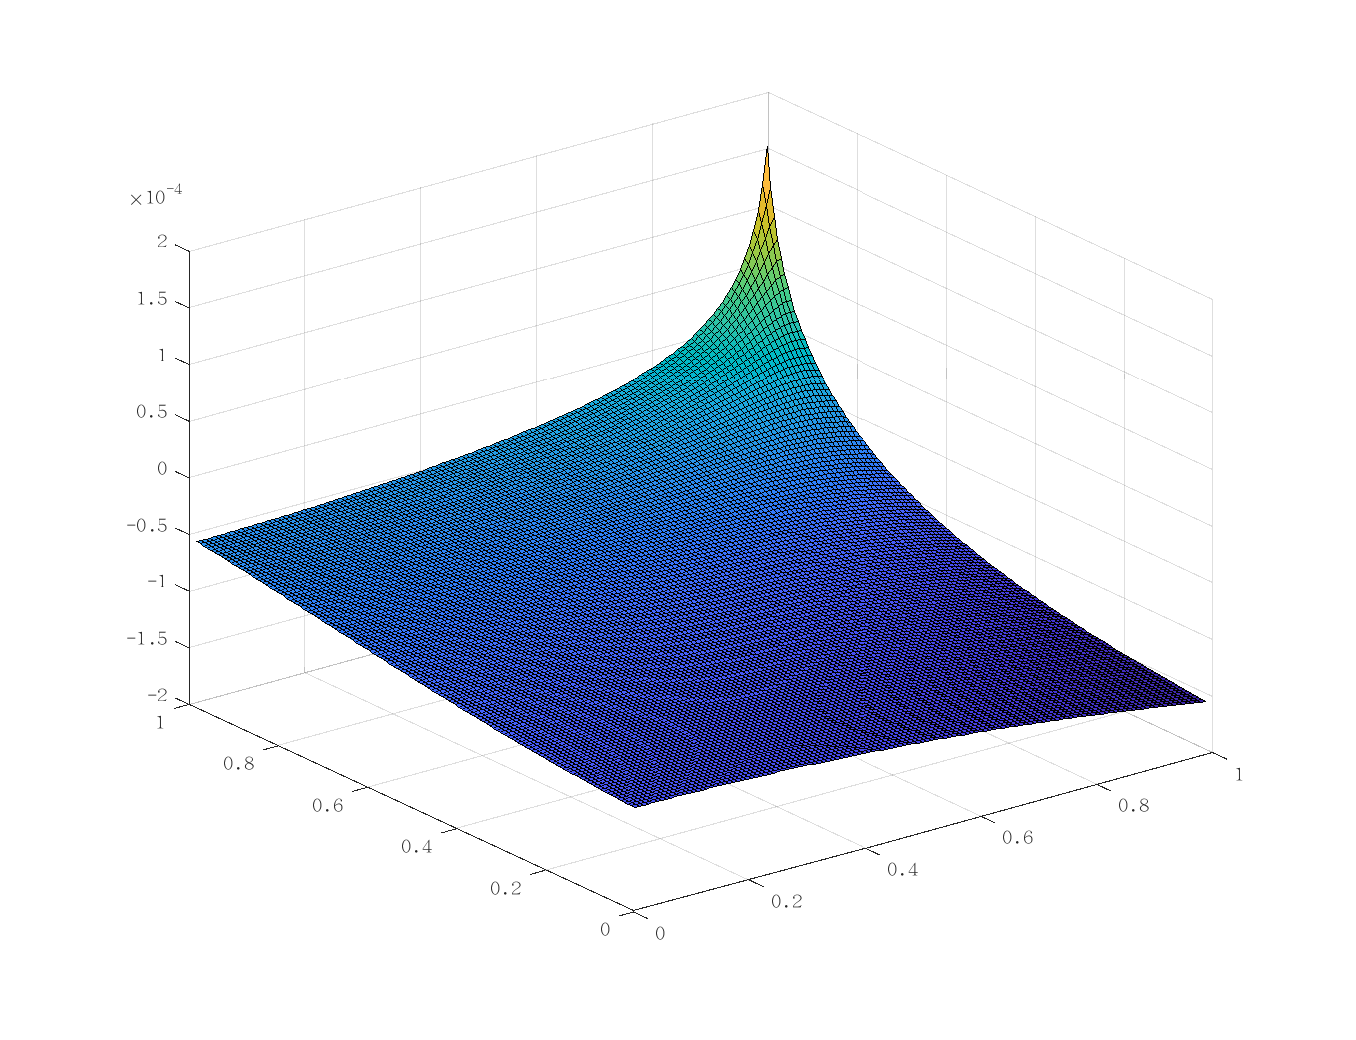
\includegraphics[width=0.95\linewidth]{figure/error_problem1_N_r_n=128.eps}
    \caption*{$n=128$}
  \end{minipage}
\end{figure}

可以看到,在Neumann条件下,格点越靠近$(1,1)$,计算误差越大,这与$u$的函数值、导数值分布有关。用$1,2,\infty$范数作误差估计,如下表。

\begin{table}[H]
  \centering
  \begin{tabular}{c|cccc|c}
  \textbf{$n$}        & 16                   & 32                   & 64                   & 128                  & 收敛率 \\ \hline
  $1$-norm error      & $1.90\times 10^{-3}$ & $7.52\times 10^{-4}$ & $2.71\times 10^{-4}$ & $9.02\times 10^{-5}$ & $1.59$\\
  $2$-norm error      & $2.28\times 10^{-3}$ & $8.48\times 10^{-4}$ & $2.93\times 10^{-4}$ & $9.48\times 10^{-5}$ & $1.63$\\
  $\infty$-norm error & $5.02\times 10^{-3}$ & $1.68\times 10^{-3}$ & $5.23\times 10^{-4}$ & $1.55\times 10^{-4}$ & $1.75$
  \end{tabular}
\end{table}

再用(2)中函数$u_2$导出相应的Neumann边值问题,求解得到误差与收敛率如下表。

\begin{table}[H]
  \centering
  \begin{tabular}{c|cccc|c}
  \textbf{$n$}        & 16                   & 32                   & 64                   & 128                  & 收敛率 \\ \hline
  $1$-norm error      & $5.78\times 10^{-2}$ & $2.23\times 10^{-2}$ & $8.02\times 10^{-3}$ & $2.67\times 10^{-3}$ & $1.59$\\
  $2$-norm error      & $7.31\times 10^{-2}$ & $2.62\times 10^{-2}$ & $8.93\times 10^{-3}$ & $2.87\times 10^{-3}$ & $1.64$\\
  $\infty$-norm error & $2.20\times 10^{-1}$ & $7.03\times 10^{-2}$ & $2.03\times 10^{-2}$ & $5.75\times 10^{-3}$ & $1.82$
  \end{tabular}
\end{table}

再用(3)中函数$u_3$导出相应的Neumann边值问题,求解得到误差与收敛率如下表。

\begin{table}[H]
  \centering
  \begin{tabular}{c|cccc|c}
  \textbf{$n$}        & 16                   & 32                   & 64                   & 128                  & 收敛率 \\ \hline
  $1$-norm error      & $18.1$ & $8.38$ & $3.19$ & $1.07$ & $1.57$\\
  $2$-norm error      & $19.1$ & $8.73$ & $3.28$ & $1.10$ & $1.58$\\
  $\infty$-norm error & $27.6$ & $11.9$ & $4.26$ & $1.37$ & $1.64$
  \end{tabular}
\end{table}

上述三个测试函数与2阶收敛的理论结果不吻合。这可能是因为在Neumann条件下,所求解的矩阵比较病态,而且需要人为添加额外条件,导致方程组的求解误差较大。

\subsection{混合条件}

考虑由精确解$u_1(x,y)=e^{\sin x+y}$导出的混合边值问题
\begin{equation}
  \left\{
    \begin{array}{l}
      -\Delta u = -(1-\sin x+\cos^2 x)e^{\sin x + y},\quad x\in\Omega, \\
      u|_{x=0}=e^{y},\\
      u|_{x=1}=e^{y+\sin 1},\\
      \frac{\partial u}{\partial \mathbf{n}}|_{y=0}=-e^{\sin x},\\
      \frac{\partial u}{\partial \mathbf{n}}|_{y=1}=e^{\sin x+1}
    \end{array}
  \right. .
\end{equation}

用$n=16,32,64,128$的网格求解,并与真实解作差,所得各点残差的图像如下。

\begin{figure}[htbp]
  \centering
  \begin{minipage}[t]{0.24\linewidth}
      \centering
      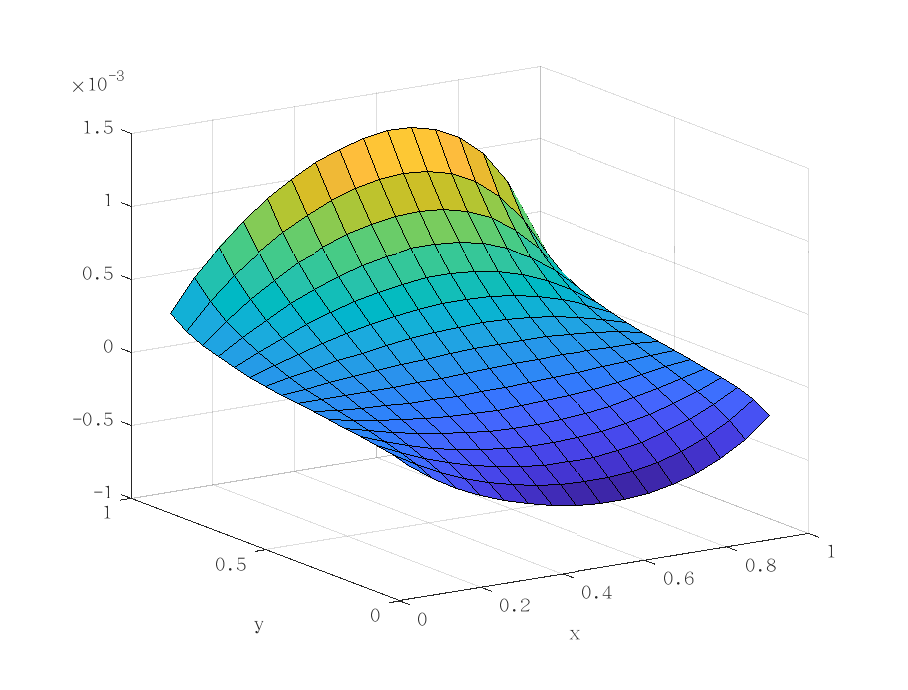
\includegraphics[width=0.95\linewidth]{figure/error_problem1_m_r_n=16.eps}
      \caption*{$n=16$}
  \end{minipage}
  \begin{minipage}[t]{0.24\linewidth}
    \centering
    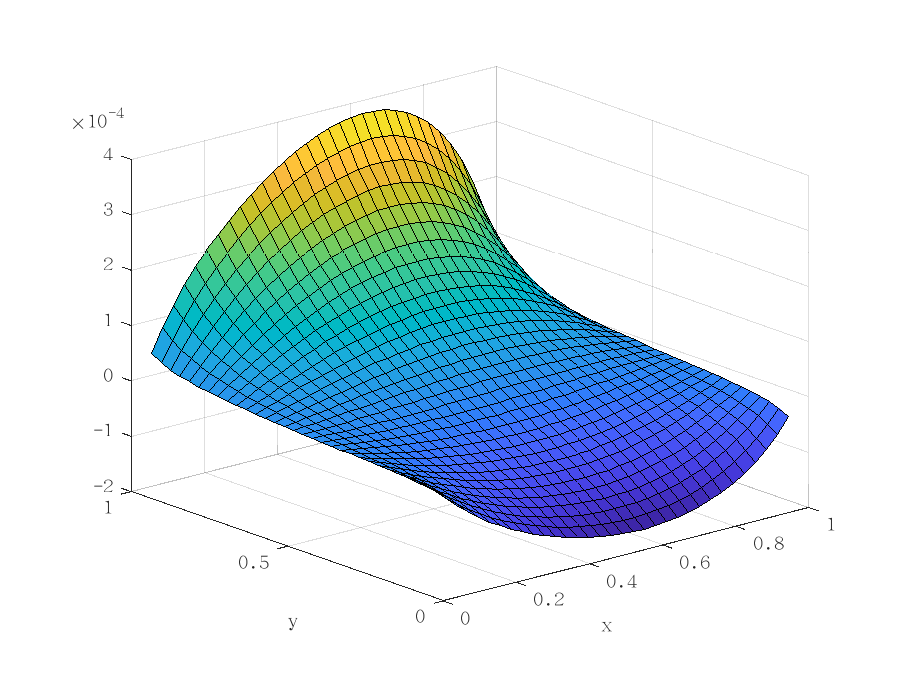
\includegraphics[width=0.95\linewidth]{figure/error_problem1_m_r_n=32.eps}
    \caption*{$n=32$}
  \end{minipage}
  \begin{minipage}[t]{0.24\linewidth}
    \centering
    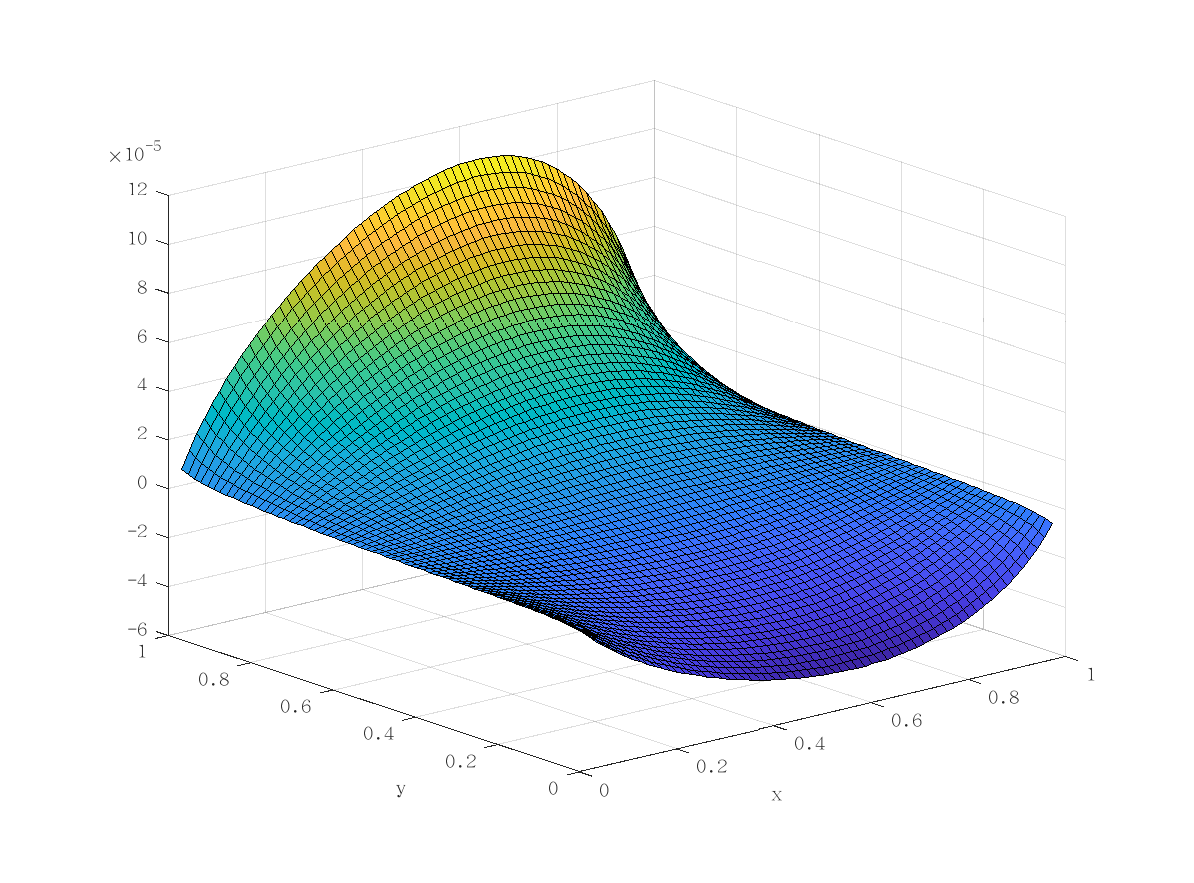
\includegraphics[width=0.95\linewidth]{figure/error_problem1_m_r_n=64.eps}
    \caption*{$n=64$}
  \end{minipage}
  \begin{minipage}[t]{0.24\linewidth}
    \centering
    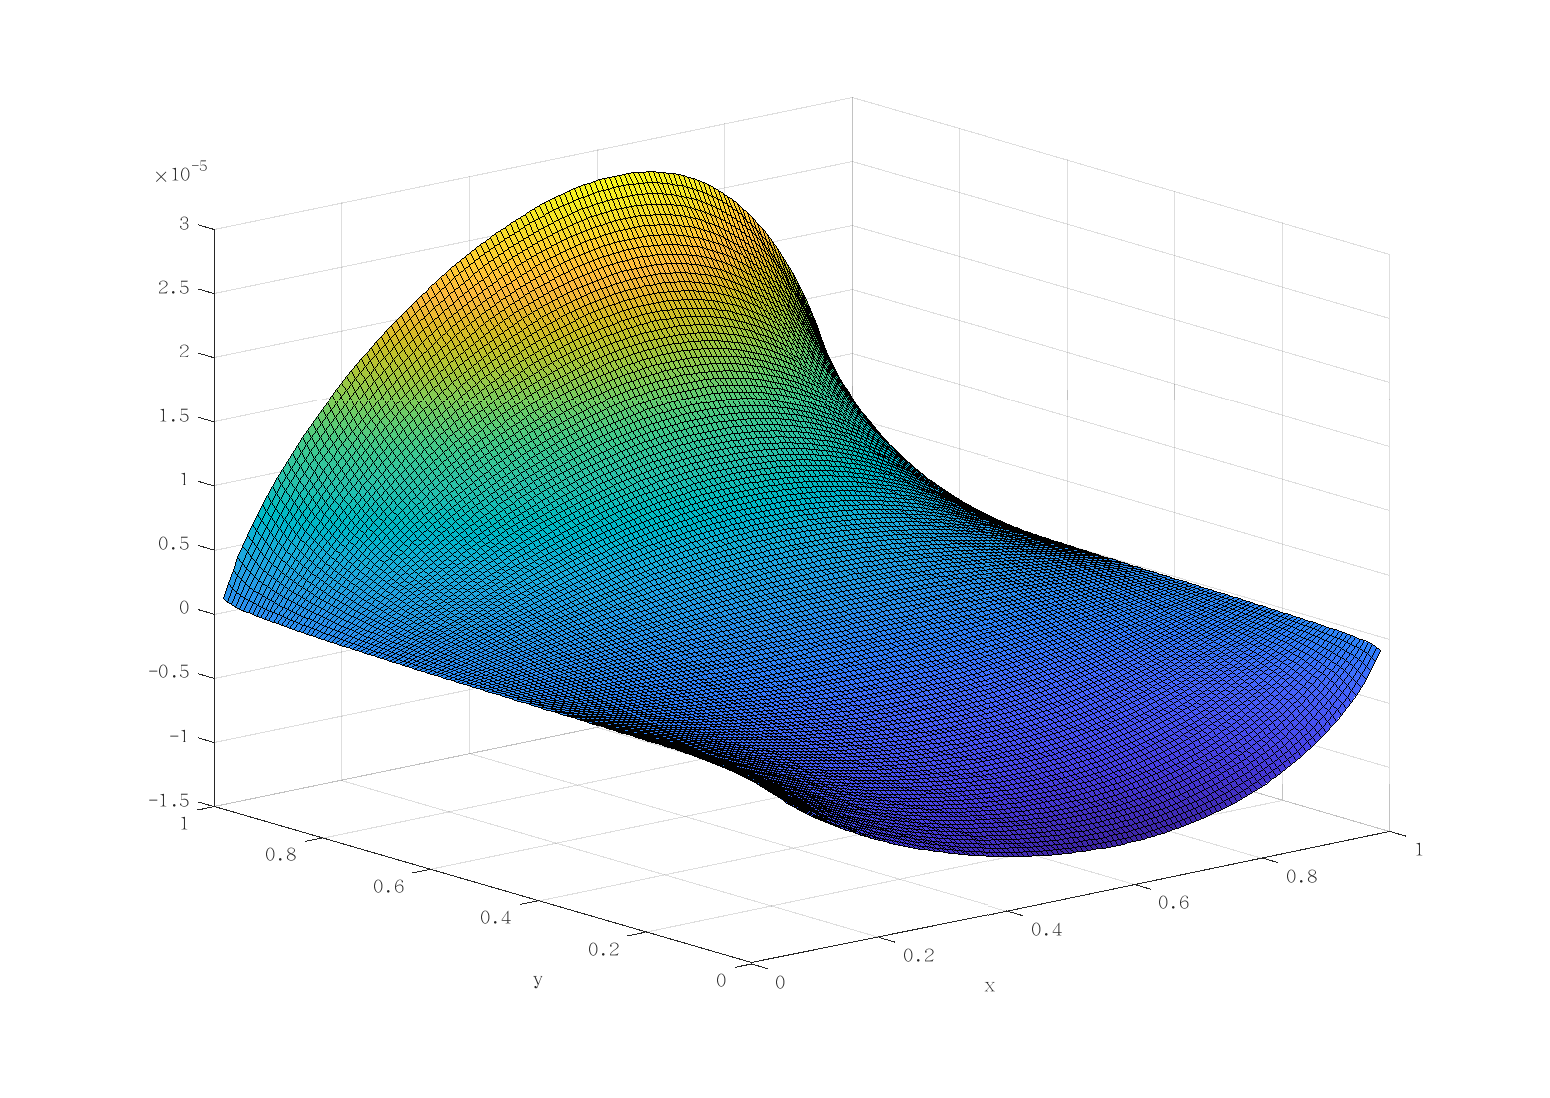
\includegraphics[width=0.95\linewidth]{figure/error_problem1_m_r_n=128.eps}
    \caption*{$n=128$}
  \end{minipage}
\end{figure}

可以看到,越靠近Dirichlet条件下的边界,求解误差越小。用$1,2,\infty$范数作误差估计,如下表。

\begin{table}[H]
  \centering
  \begin{tabular}{c|cccc|c}
  \textbf{$n$}        & 16                   & 32                   & 64                   & 128                  & 收敛率 \\ \hline
  $1$-norm error      & $3.25\times 10^{-4}$ & $8.80\times 10^{-5}$ & $2.29\times 10^{-5}$ & $5.86\times 10^{-6}$ & $1.97$\\
  $2$-norm error      & $4.37\times 10^{-4}$ & $1.21\times 10^{-4}$ & $3.20\times 10^{-5}$ & $8.22\times 10^{-6}$ & $1.96$\\
  $\infty$-norm error & $1.29\times 10^{-3}$ & $3.86\times 10^{-4}$ & $1.06\times 10^{-4}$ & $2.79\times 10^{-5}$ & $1.93$
  \end{tabular}
\end{table}

再用(2)中函数$u_2$导出相应的混合边值问题,在$x=0$与$x=1$边界上给Dirichlet条件,在$y=0$与$y=1$边界上给Neumann条件,求解得到误差与收敛率如下表。

\begin{table}[H]
  \centering
  \begin{tabular}{c|cccc|c}
  \textbf{$n$}        & 16                   & 32                   & 64                   & 128                  & 收敛率 \\ \hline
  $1$-norm error      & $5.73\times 10^{-3}$ & $1.65\times 10^{-3}$ & $4.41\times 10^{-4}$ & $1.14\times 10^{-4}$ & $1.95$\\
  $2$-norm error      & $8.02\times 10^{-3}$ & $2.36\times 10^{-3}$ & $6.39\times 10^{-4}$ & $1.66\times 10^{-4}$ & $1.95$\\
  $\infty$-norm error & $3.06\times 10^{-2}$ & $9.89\times 10^{-3}$ & $2.83\times 10^{-3}$ & $7.58\times 10^{-4}$ & $1.90$
  \end{tabular}
\end{table}

再用(3)中函数$u_3$导出相应的混合边值问题,在$x=0$与$x=1$边界上给Dirichlet条件,在$y=0$与$y=1$边界上给Neumann条件,求解得到误差与收敛率如下表。

\begin{table}[H]
  \centering
  \begin{tabular}{c|cccc|c}
  \textbf{$n$}        & 16                   & 32                   & 64                   & 128                  & 收敛率 \\ \hline
  $1$-norm error      & $3.92\times 10^{-1}$ & $1.04\times 10^{-1}$ & $2.68\times 10^{-2}$ & $6.77\times 10^{-3}$ & $1.98$\\
  $2$-norm error      & $3.97\times 10^{-1}$ & $1.07\times 10^{-1}$ & $2.76\times 10^{-2}$ & $6.99\times 10^{-3}$ & $1.98$\\
  $\infty$-norm error & $4.48\times 10^{-1}$ & $1.22\times 10^{-1}$ & $3.18\times 10^{-2}$ & $8.09\times 10^{-3}$ & $1.97$
  \end{tabular}
\end{table}

上述三个测试函数与2阶收敛的理论结果吻合。

\section{不规则边界}

在本节中,我们求解不规则区域$\Omega\setminus \mathbb{D}$中的Poisson方程。其中$\Omega$与上一节相同,$\mathbb{D}$是一个自定义的闭圆盘,它被完全包含在$\Omega$内,且与$\Omega$的边界至少相隔$3$个格点。

\subsection{Dirichlet条件}

考虑由精确解$u_1(x,y)=e^{\sin x+y}$导出的Dirichlet边值问题,其中$\mathbb{D}=\mathbb{D}((0.4,0.4),0.2)$:
\begin{equation}
  \left\{
    \begin{array}{l}
      -\Delta u = -(1-\sin x+\cos^2 x)e^{\sin x + y},\quad x\in\Omega\setminus\mathbb{D} \\
      u|_{\partial (\Omega\setminus\mathbb{D})}=e^{\sin x + y}
    \end{array}
  \right. .
\end{equation}

用$n=16,32,64,128$的网格求解,并与真实解作差,所得各点残差的图像如下。

\begin{figure}[htbp]
  \centering
  \begin{minipage}[t]{0.24\linewidth}
      \centering
      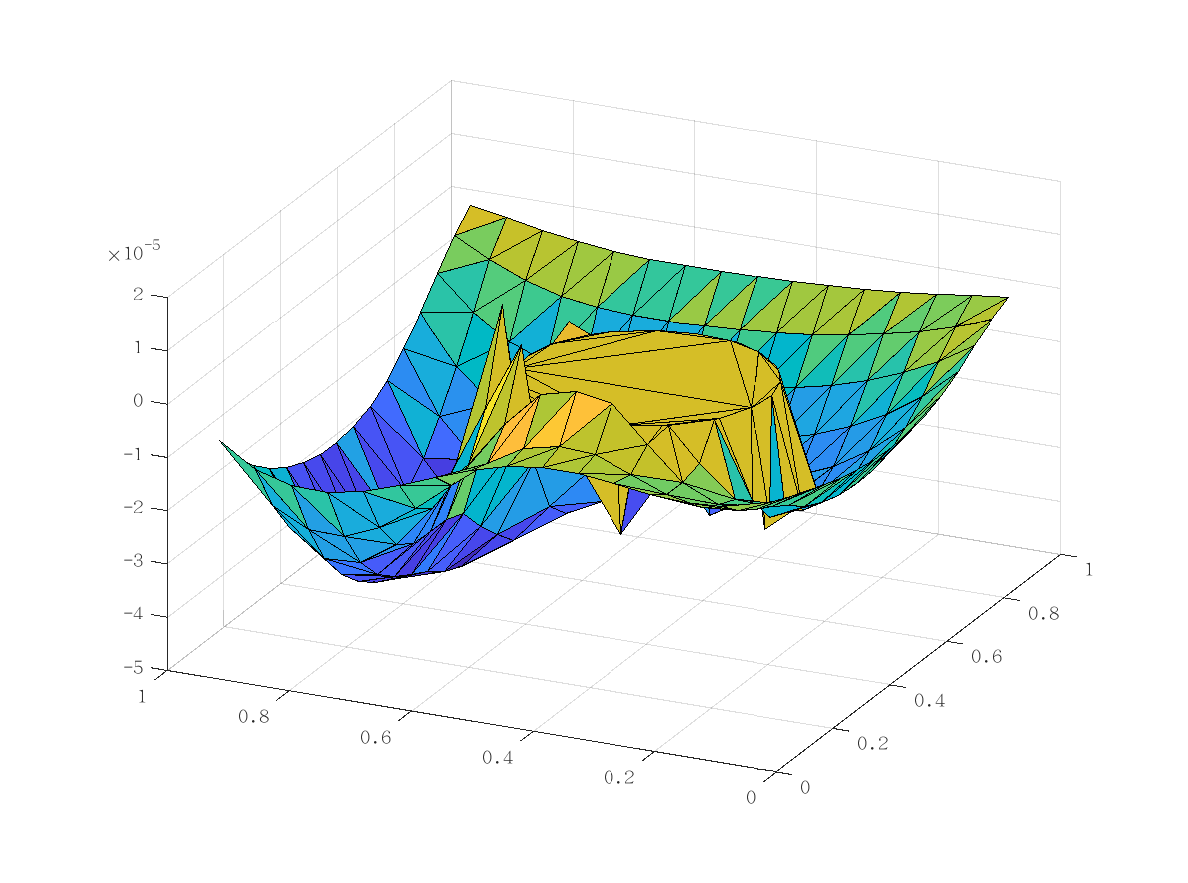
\includegraphics[width=0.95\linewidth]{figure/error_problem1_D_ir_n=16.eps}
      \caption*{$n=16$}
  \end{minipage}
  \begin{minipage}[t]{0.24\linewidth}
    \centering
    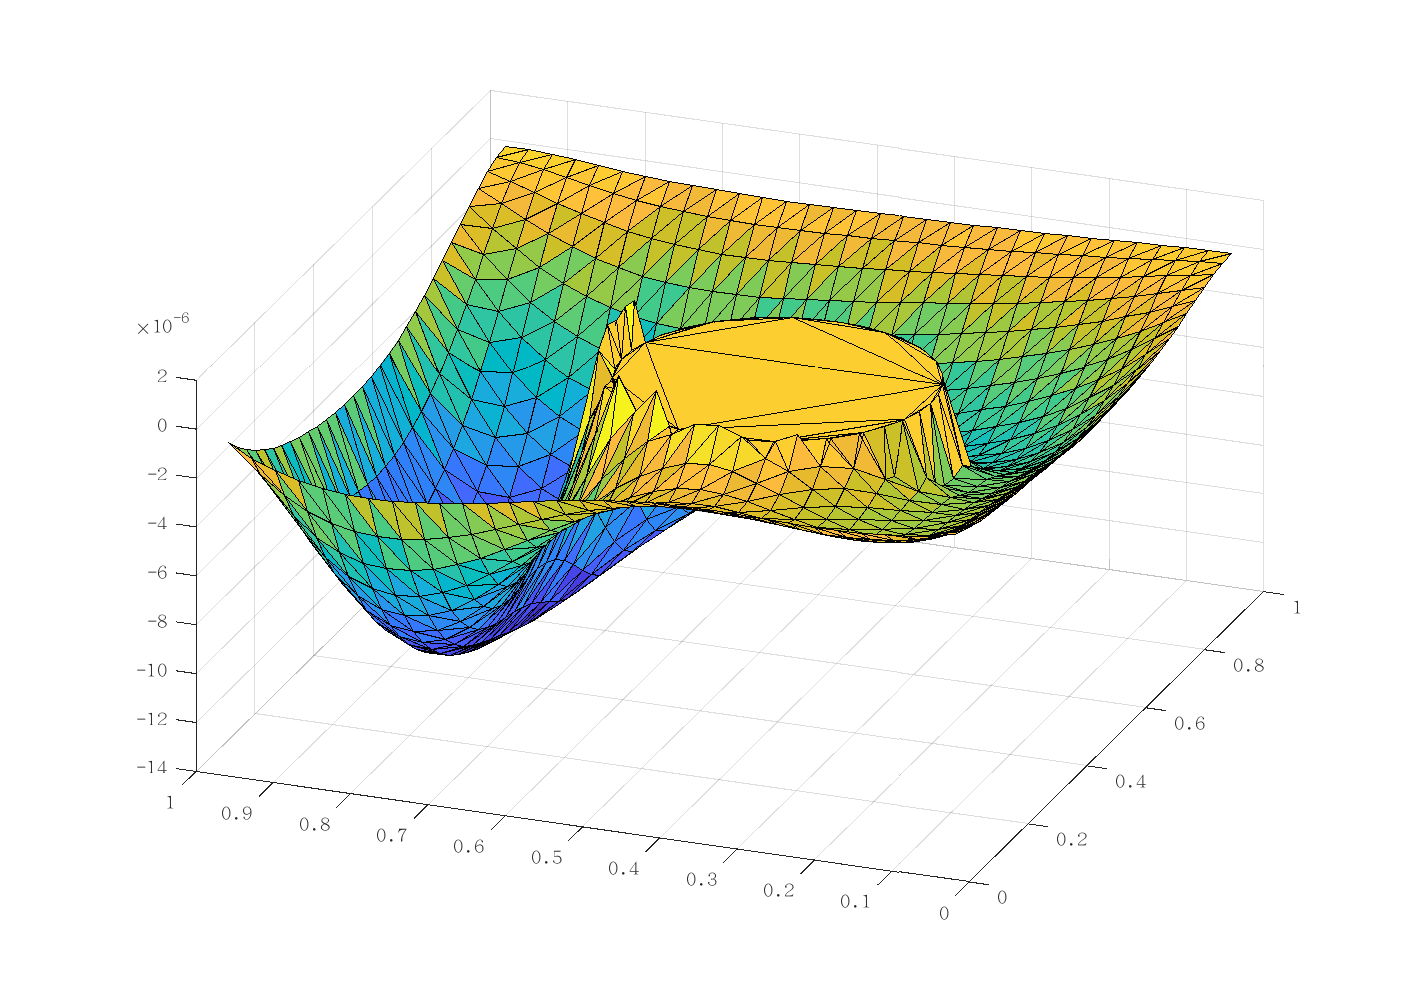
\includegraphics[width=0.95\linewidth]{figure/error_problem1_D_ir_n=32.eps}
    \caption*{$n=32$}
  \end{minipage}
  \begin{minipage}[t]{0.24\linewidth}
    \centering
    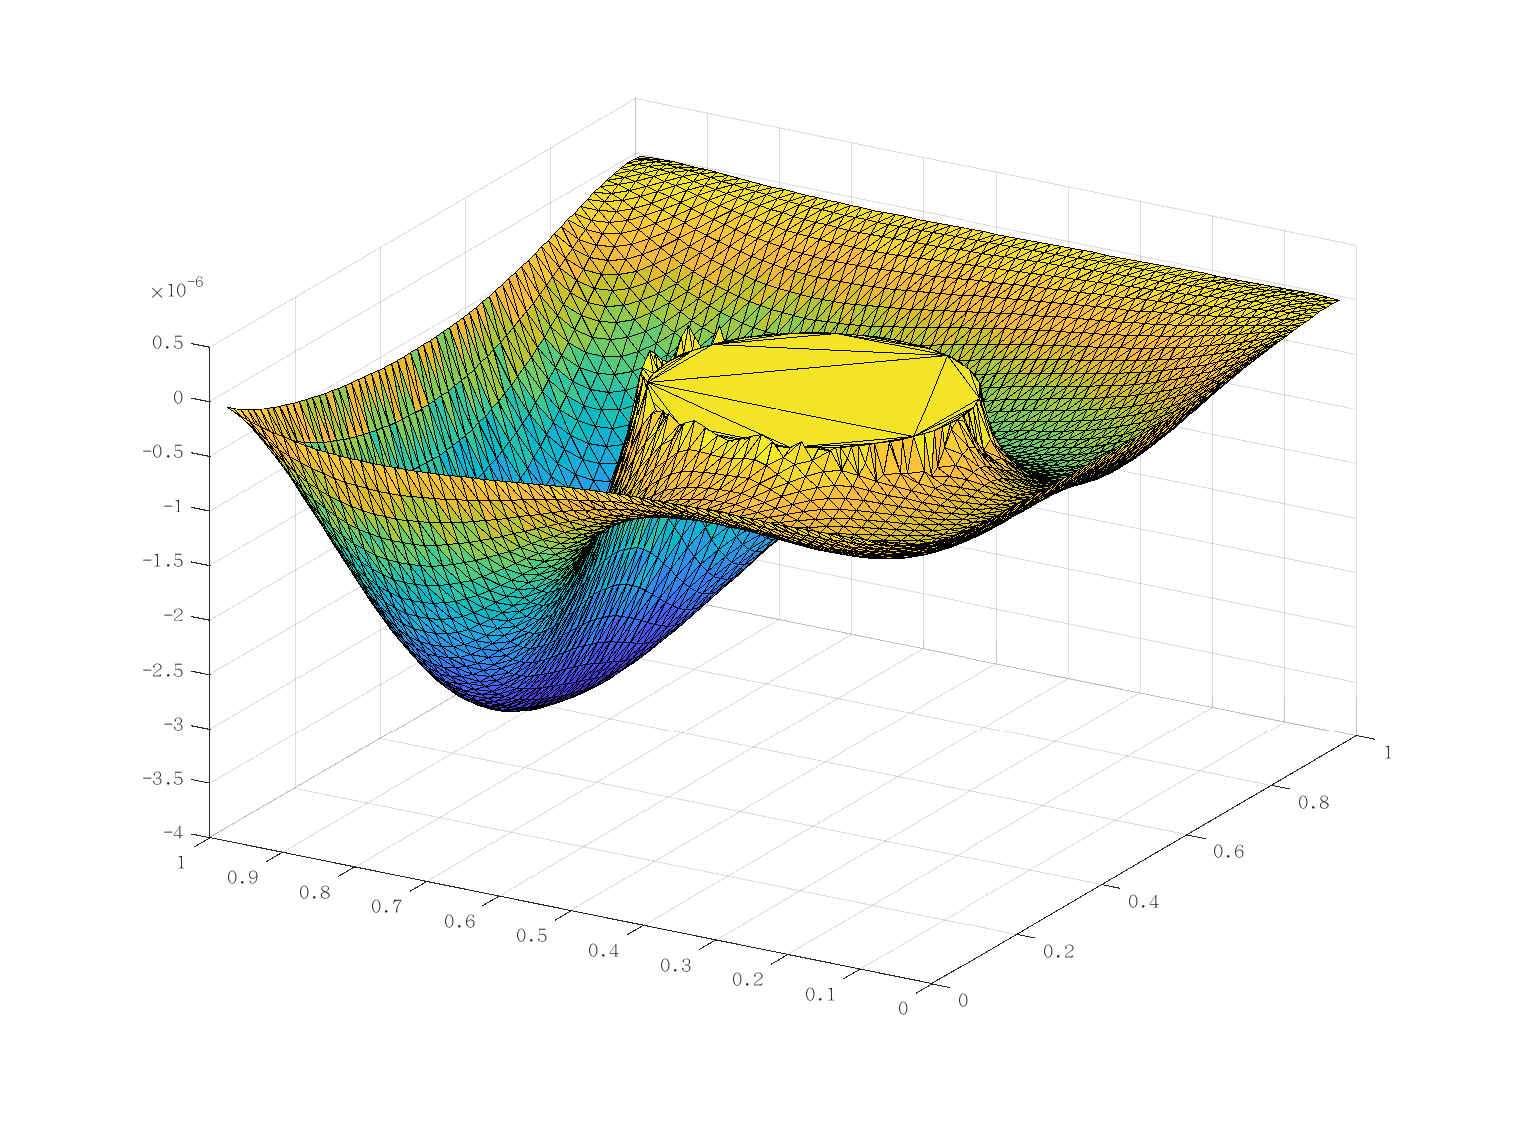
\includegraphics[width=0.95\linewidth]{figure/error_problem1_D_ir_n=64.eps}
    \caption*{$n=64$}
  \end{minipage}
  \begin{minipage}[t]{0.24\linewidth}
    \centering
    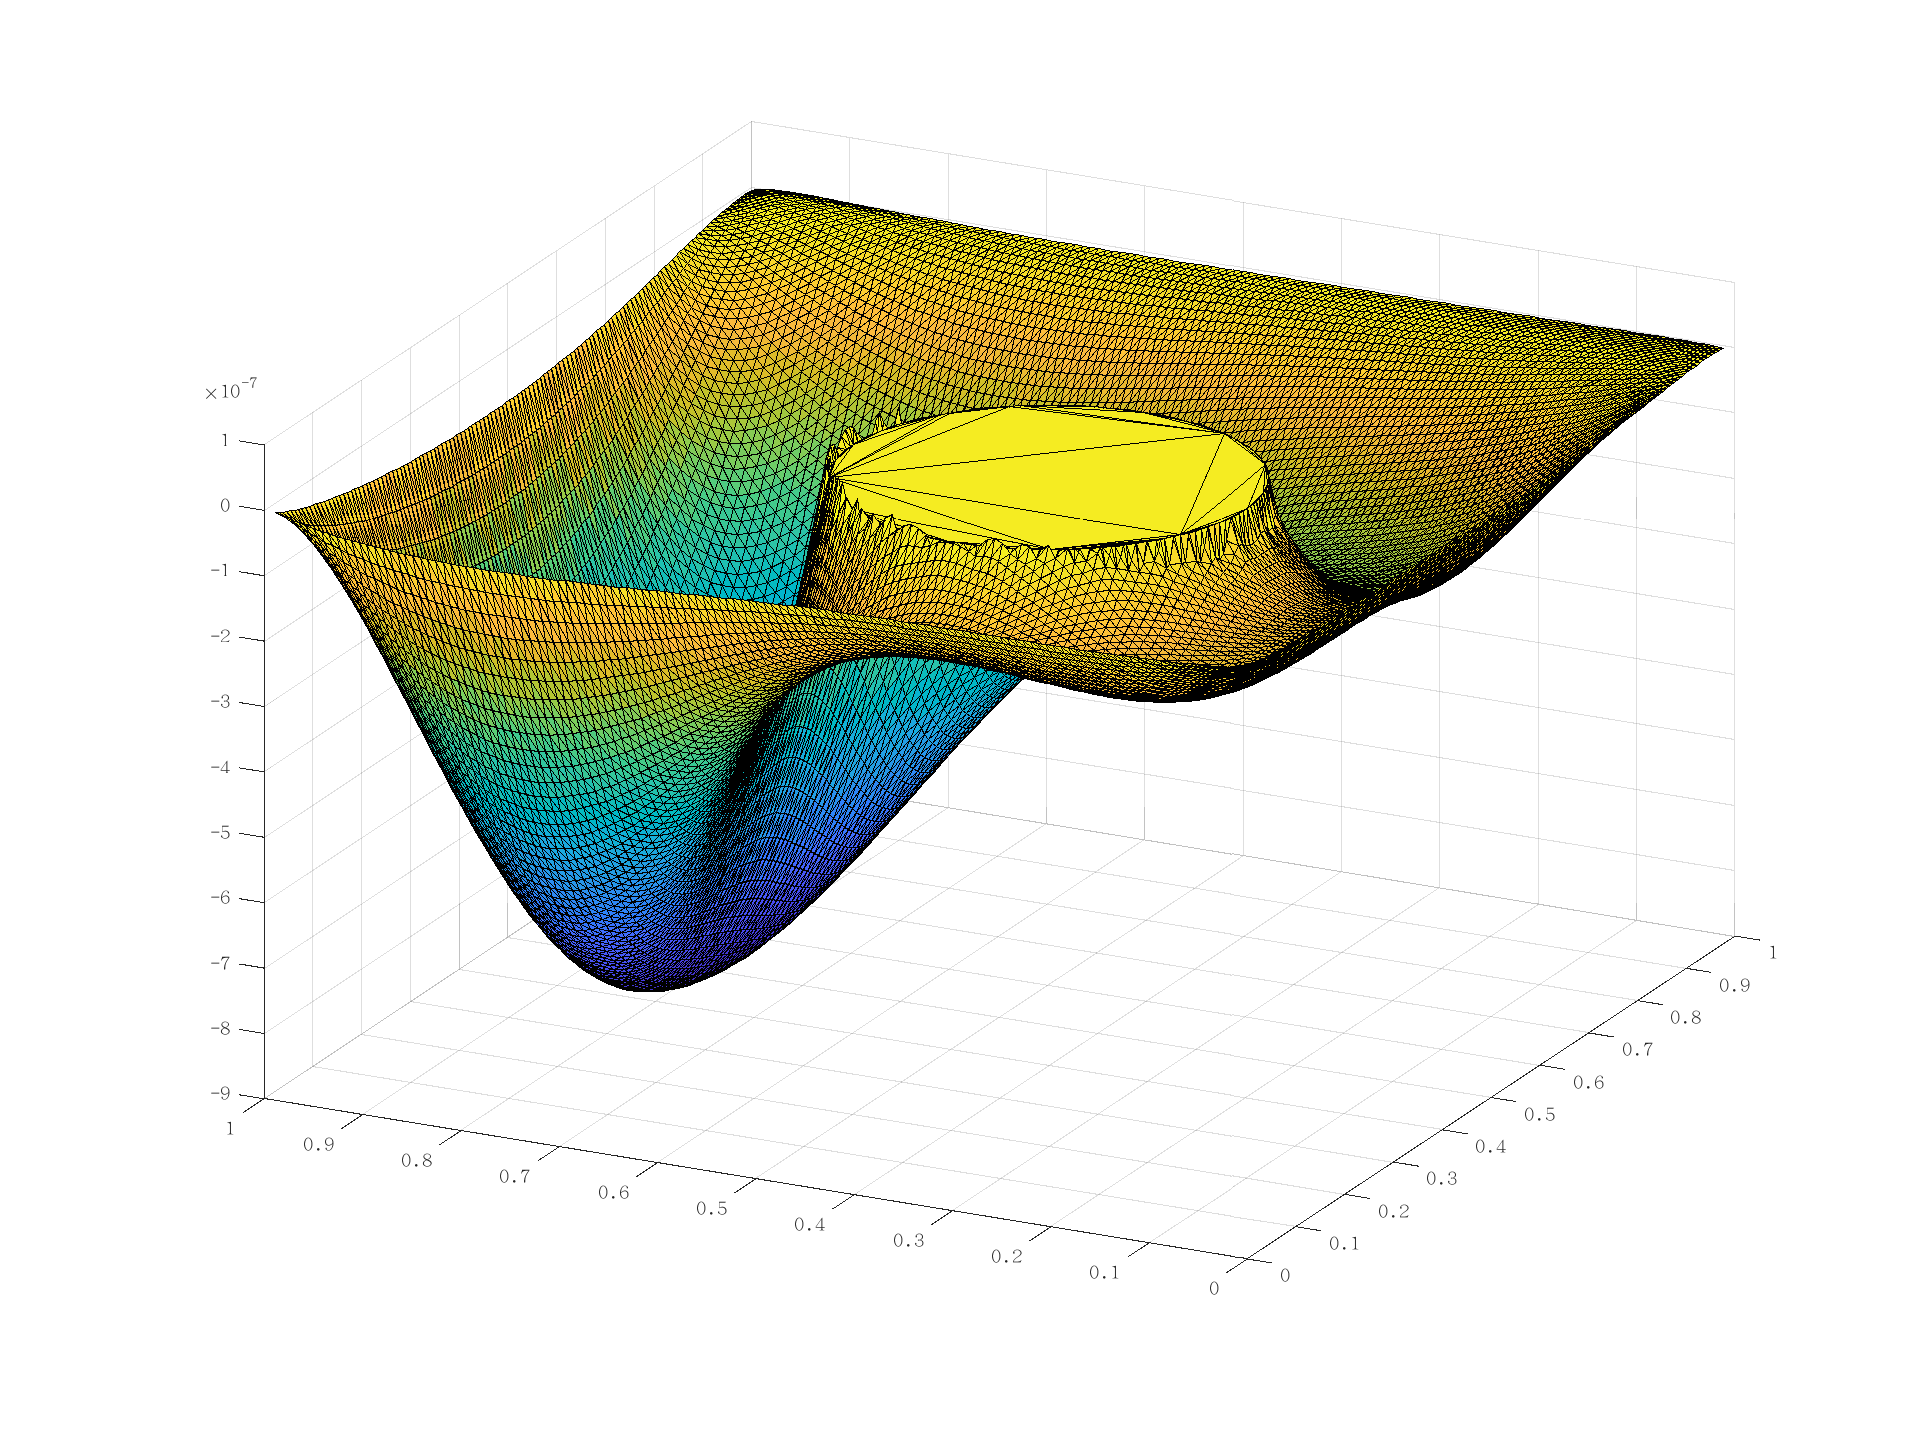
\includegraphics[width=0.95\linewidth]{figure/error_problem1_D_ir_n=128.eps}
    \caption*{$n=128$}
  \end{minipage}
\end{figure}

可以看到,越靠近边界,求解误差越小。用$1,2,\infty$范数作误差估计,如下表。

\begin{table}[H]
  \centering
  \begin{tabular}{c|cccc|c}
  \textbf{$n$}        & 16                   & 32                   & 64                   & 128                  & 收敛率 \\ \hline
  $1$-norm error      & $1.74\times 10^{-5}$ & $4.40\times 10^{-6}$ & $1.08\times 10^{-6}$ & $2.72\times 10^{-7}$ & $2.00$\\
  $2$-norm error      & $2.22\times 10^{-5}$ & $5.71\times 10^{-6}$ & $1.45\times 10^{-6}$ & $3.66\times 10^{-7}$ & $1.98$\\
  $\infty$-norm error & $4.76\times 10^{-5}$ & $1.32\times 10^{-5}$ & $3.51\times 10^{-6}$ & $8.96\times 10^{-7}$ & $1.97$
  \end{tabular}
\end{table}

再用(2)中精确解$u_2$导出相应的Dirichlet边值问题,取$\mathbb{D}=\mathbb{D}((0.4,0.4),0.2)$,用数值方法求解,得到误差与收敛率如下表。

\begin{table}[H]
  \centering
  \begin{tabular}{c|cccc|c}
  \textbf{$n$}        & 16                   & 32                   & 64                   & 128                  & 收敛率 \\ \hline
  $1$-norm error      & $2.20\times 10^{-4}$ & $5.91\times 10^{-5}$ & $1.53\times 10^{-5}$ & $3.86\times 10^{-6}$ & $1.98$\\
  $2$-norm error      & $6.63\times 10^{-4}$ & $1.74\times 10^{-4}$ & $4.48\times 10^{-5}$ & $1.13\times 10^{-5}$ & $1.98$\\
  $\infty$-norm error & $3.67\times 10^{-3}$ & $9.63\times 10^{-4}$ & $2.47\times 10^{-4}$ & $6.28\times 10^{-5}$ & $1.98$
  \end{tabular}
\end{table}

再用(3)中精确解$u_3$导出相应的Dirichlet边值问题,取$\mathbb{D}=\mathbb{D}((0.5,0.5),0.25)$,用数值方法求解,得到误差与收敛率如下表。

\begin{table}[H]
  \centering
  \begin{tabular}{c|cccc|c}
  \textbf{$n$}        & 16                   & 32                   & 64                   & 128                  & 收敛率 \\ \hline
  $1$-norm error      & $7.20\times 10^{-2}$ & $2.04\times 10^{-2}$ & $5.36\times 10^{-3}$ & $1.37\times 10^{-3}$ & $1.97$\\
  $2$-norm error      & $9.19\times 10^{-2}$ & $2.52\times 10^{-2}$ & $6.55\times 10^{-3}$ & $1.67\times 10^{-3}$ & $1.97$\\
  $\infty$-norm error & $1.65\times 10^{-1}$ & $4.50\times 10^{-2}$ & $1.18\times 10^{-2}$ & $3.00\times 10^{-3}$ & $1.98$
  \end{tabular}
\end{table}

上面三个测试函数符合2阶收敛的理论结果。

\subsection{Neumann条件}

考虑由精确解$u_1(x,y)=e^{\sin x+y}$导出的Neumann边值问题
\begin{equation}
  \left\{
    \begin{array}{l}
      -\Delta u = -(1-\sin x+\cos^2 x)e^{\sin x + y},\quad x\in\Omega\setminus\mathbb{D}, \\
      \frac{\partial u}{\partial \mathbf{n}}|_{x=0}=-e^{y}, \quad \frac{\partial u}{\partial \mathbf{n}}|_{x=1}=\cos 1 \cdot e^{\sin 1 + y},\\
      \frac{\partial u}{\partial \mathbf{n}}|_{y=0}=-e^{\sin x}, \quad \frac{\partial u}{\partial \mathbf{n}}|_{y=1}=e^{\sin x+1},\\
      -\frac{\partial u}{\partial \mathbf{n}}|_{\partial \mathbb{D}}=\frac{x-x_0}{R}\cos x \cdot e^{\sin x+y}+\frac{y-y_0}{R}e^{\sin x +y}
    \end{array}
  \right. .
\end{equation}

其中$(x_0,y_0)$是$\mathbb{D}$的中心,$R$是$\mathbb{D}$的半径。取$\mathbb{D}=\mathbb{D}((0.5,0.5),0.2)$,用$n=16,32,64,128$的网格求解,将数值解加上常数后与真实解作差,得到各点残差图像如下。

\begin{figure}[htbp]
  \centering
  \begin{minipage}[t]{0.24\linewidth}
      \centering
      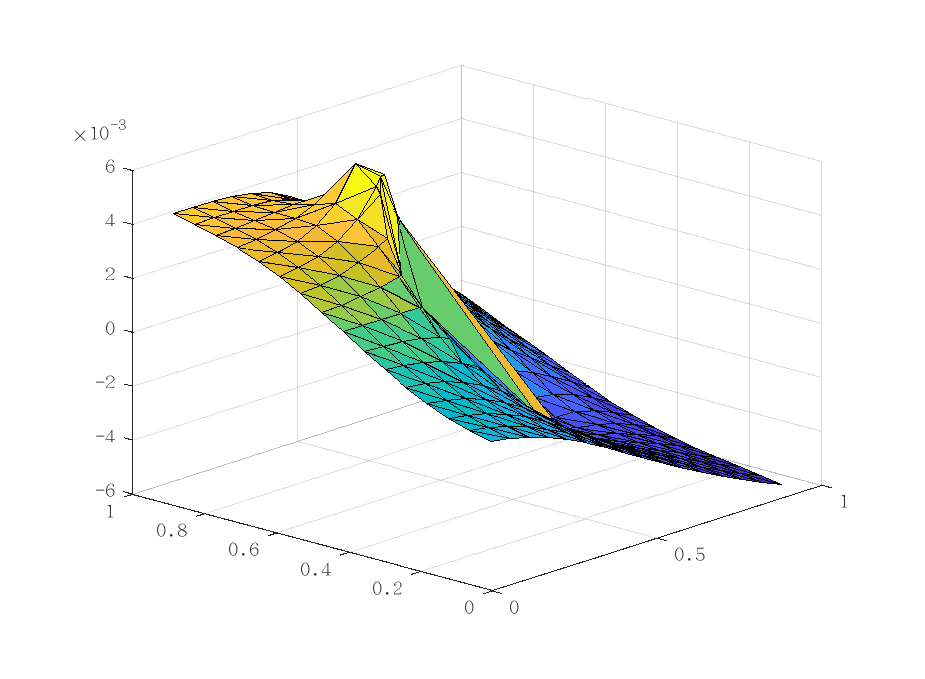
\includegraphics[width=0.95\linewidth]{figure/error_problem1_N_ir_n=16.eps}
      \caption*{$n=16$}
  \end{minipage}
  \begin{minipage}[t]{0.24\linewidth}
    \centering
    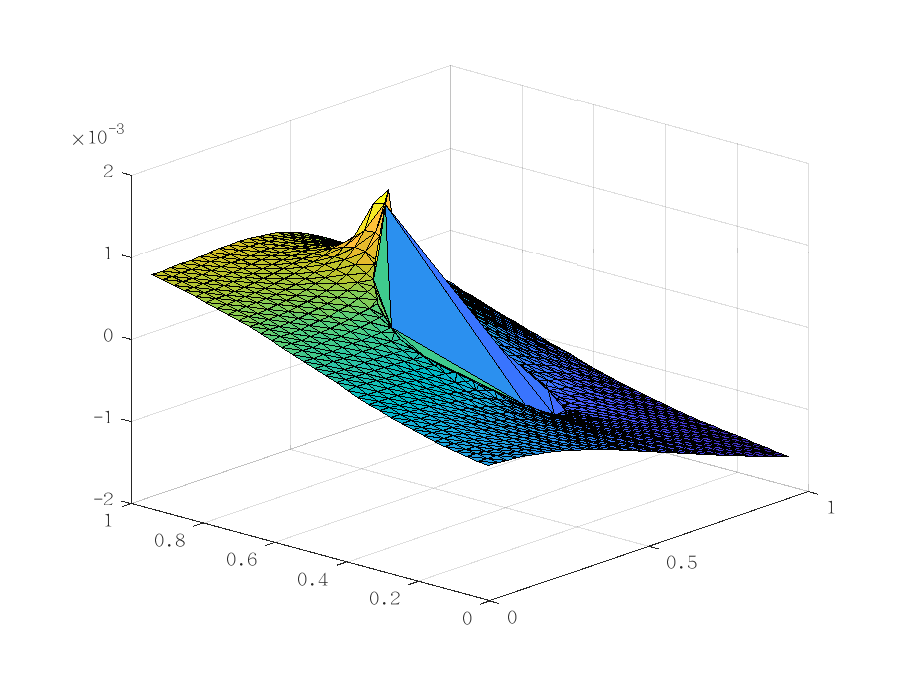
\includegraphics[width=0.95\linewidth]{figure/error_problem1_N_ir_n=32.eps}
    \caption*{$n=32$}
  \end{minipage}
  \begin{minipage}[t]{0.24\linewidth}
    \centering
    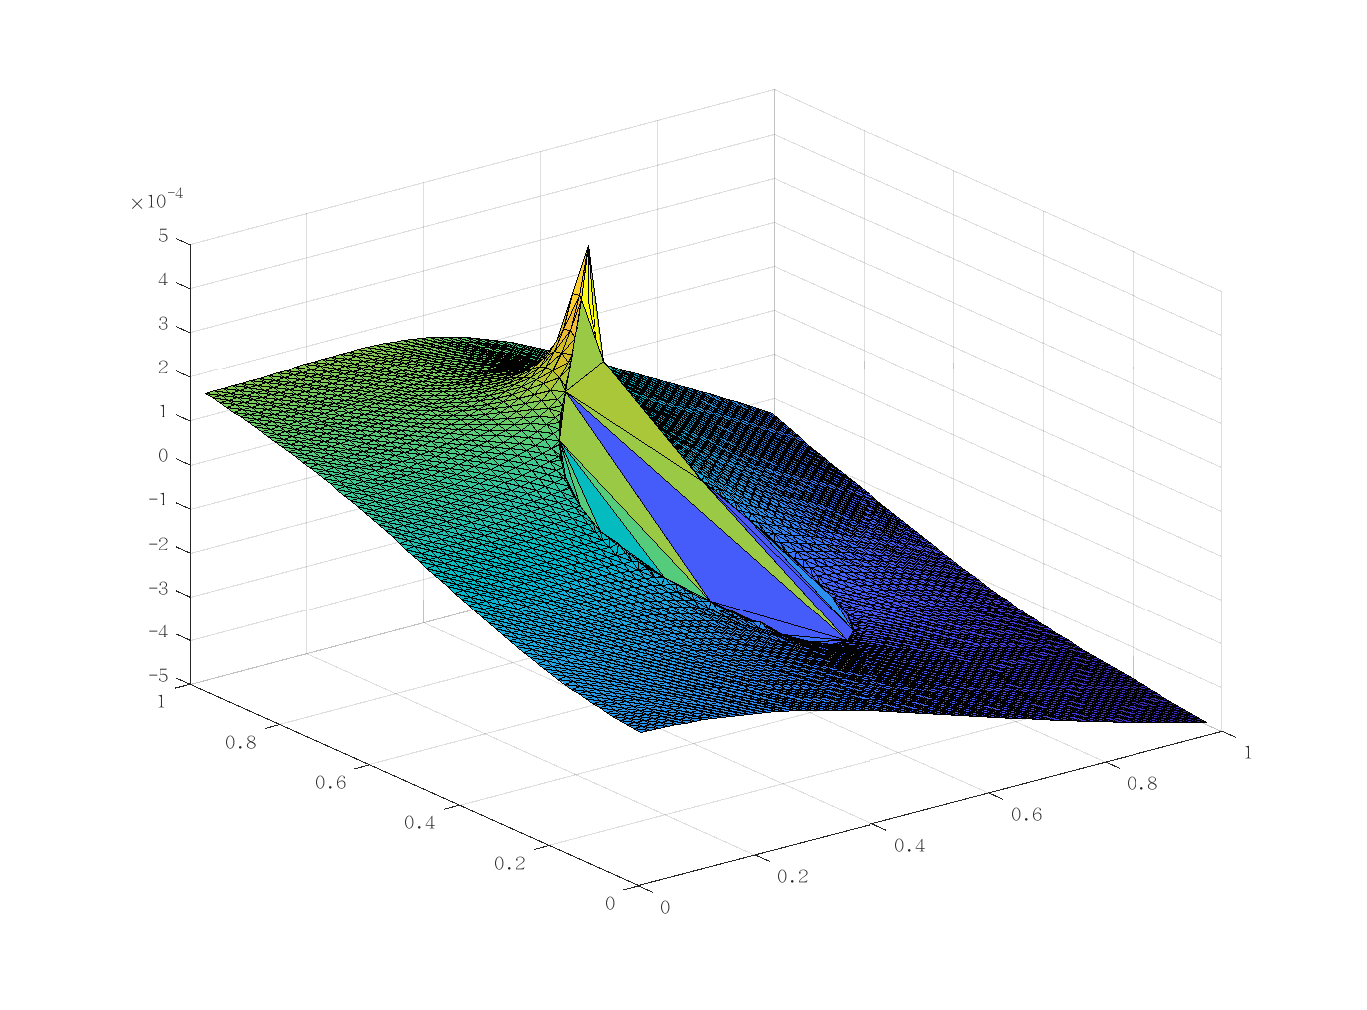
\includegraphics[width=0.95\linewidth]{figure/error_problem1_N_ir_n=64.eps}
    \caption*{$n=64$}
  \end{minipage}
  \begin{minipage}[t]{0.24\linewidth}
    \centering
    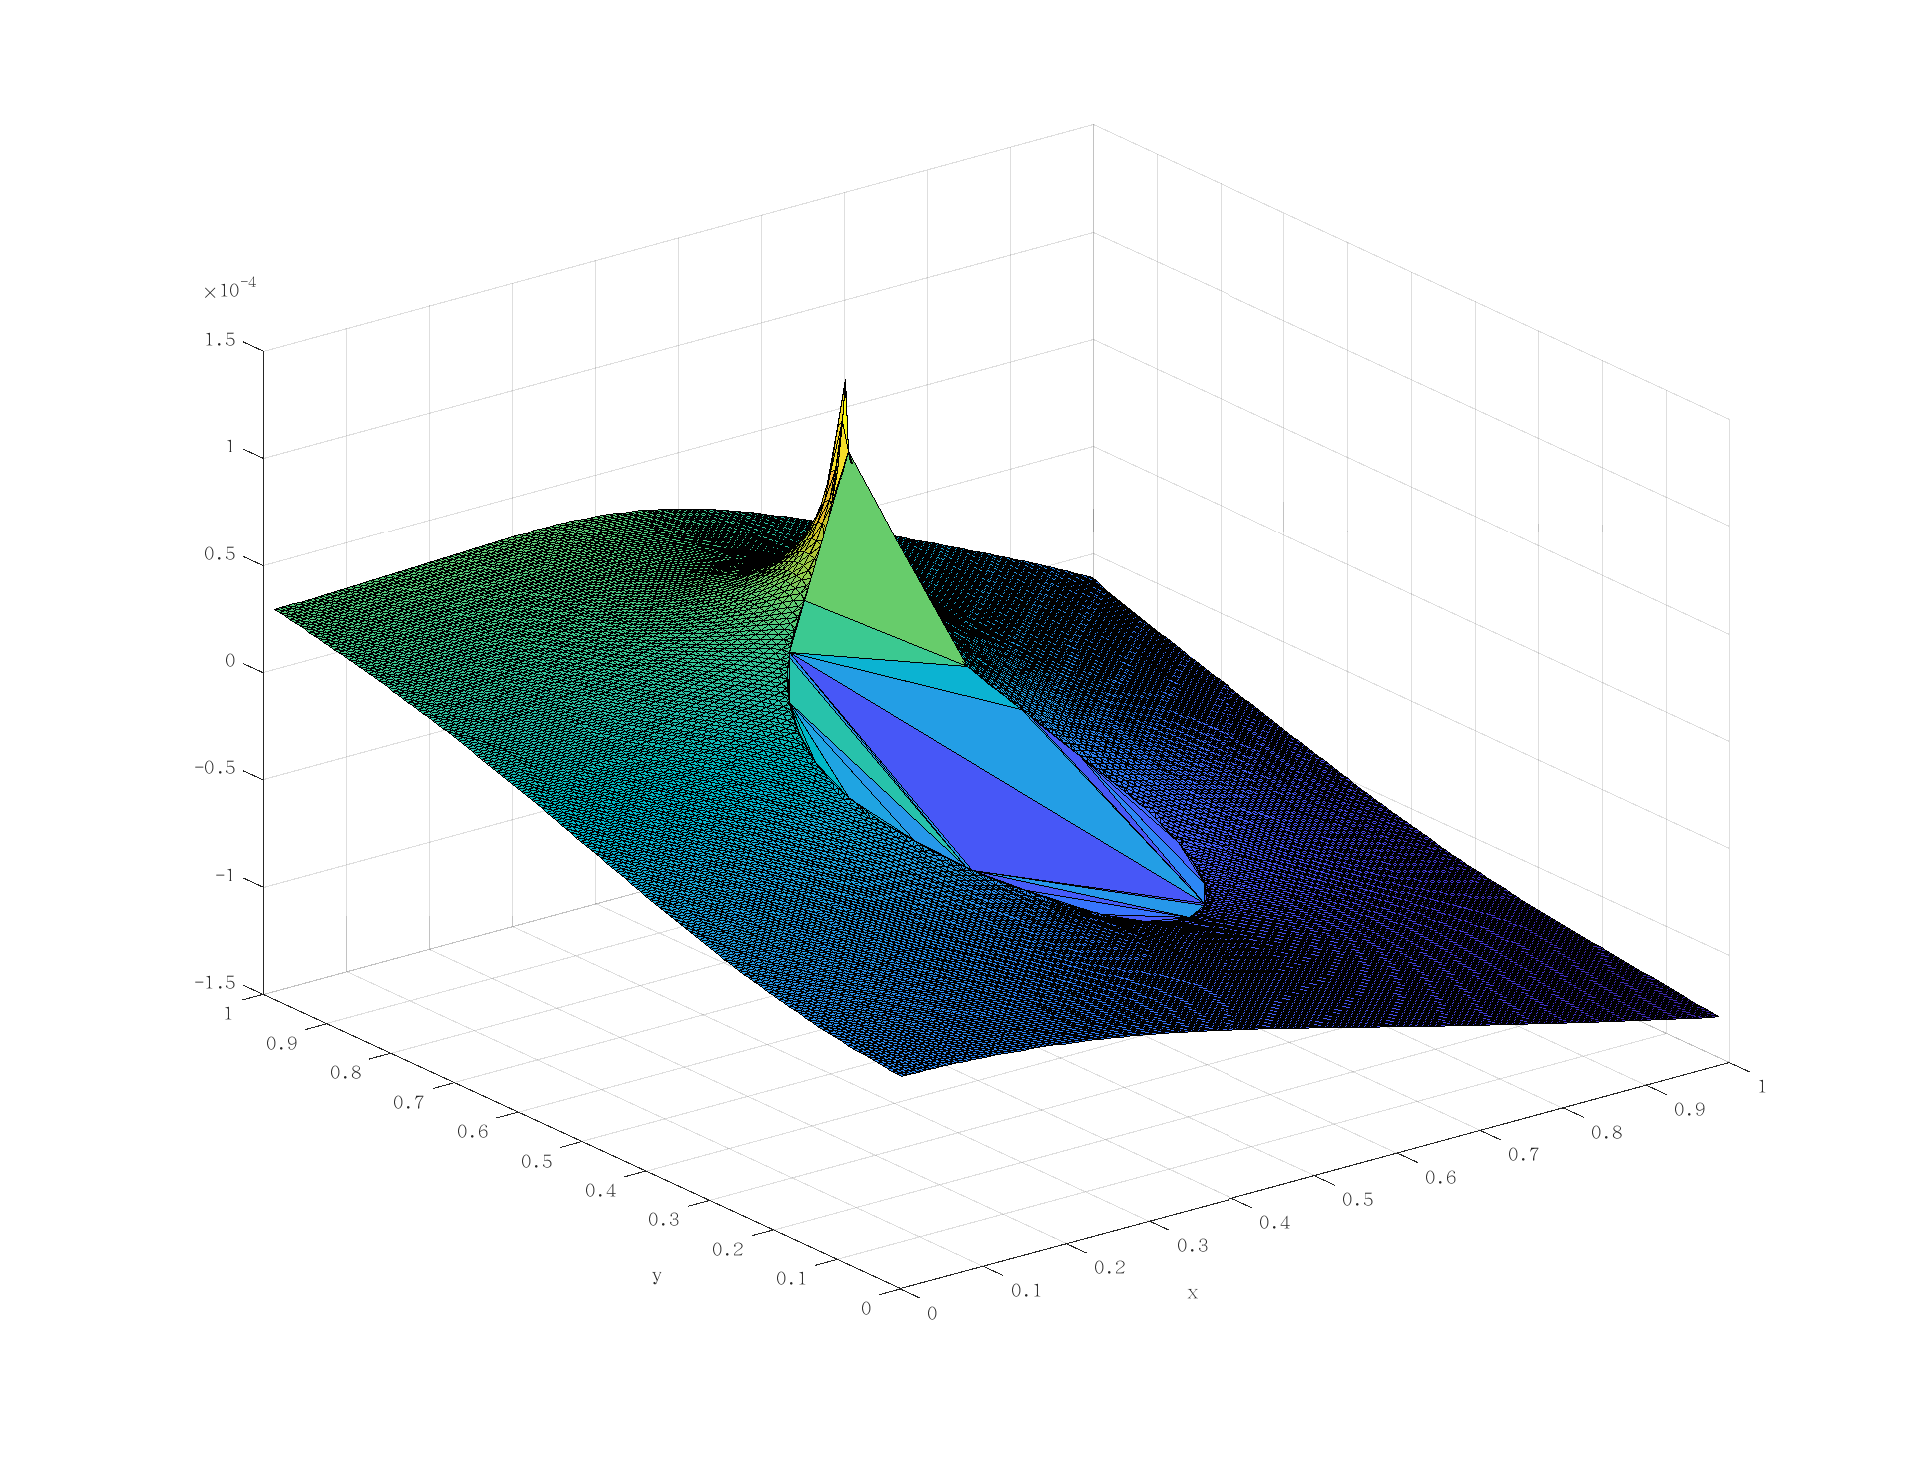
\includegraphics[width=0.95\linewidth]{figure/error_problem1_N_ir_n=128.eps}
    \caption*{$n=128$}
  \end{minipage}
\end{figure}

误差的分布几乎无规律,只能看出不规则边界上有一点附近误差非常大。用$1,2,\infty$范数作误差估计,如下表。

\begin{table}[H]
  \centering
  \begin{tabular}{c|cccc|c}
  \textbf{$n$}        & 16                   & 32                   & 64                   & 128                  & 收敛率 \\ \hline
  $1$-norm error      & $2.88\times 10^{-3}$ & $6.56\times 10^{-4}$ & $2.01\times 10^{-4}$ & $5.30\times 10^{-5}$ & $1.92$\\
  $2$-norm error      & $3.29\times 10^{-3}$ & $7.56\times 10^{-4}$ & $2.35\times 10^{-4}$ & $6.30\times 10^{-5}$ & $1.90$\\
  $\infty$-norm error & $5.96\times 10^{-3}$ & $1.57\times 10^{-3}$ & $4.83\times 10^{-4}$ & $1.29\times 10^{-4}$ & $1.91$
  \end{tabular}
\end{table}

再用(2)中精确解$u_2$导出相应的Neumann边值问题,取$\mathbb{D}=\mathbb{D}((0.45,0.5),0.25)$,用数值方法求解,得到误差与收敛率如下表。

\begin{table}[H]
  \centering
  \begin{tabular}{c|cccc|c}
  \textbf{$n$}        & 16                   & 32                   & 64                   & 128                  & 收敛率 \\ \hline
  $1$-norm error      & $9.04\times 10^{-2}$ & $2.45\times 10^{-2}$ & $6.26\times 10^{-3}$ & $1.54\times 10^{-3}$ & $2.02$\\
  $2$-norm error      & $1.08\times 10^{-1}$ & $2.94\times 10^{-2}$ & $7.71\times 10^{-3}$ & $1.91\times 10^{-3}$ & $2.01$\\
  $\infty$-norm error & $2.38\times 10^{-1}$ & $7.09\times 10^{-2}$ & $1.95\times 10^{-2}$ & $4.75\times 10^{-3}$ & $2.03$
  \end{tabular}
\end{table}

再用(3)中精确解$u_3$导出相应的Neumann边值问题,取$\mathbb{D}=\mathbb{D}((0.5,0.5),0.3)$,用数值方法求解,得到误差与收敛率如下表。

\begin{table}[H]
  \centering
  \begin{tabular}{c|cccc|c}
  \textbf{$n$}        & 16                   & 32                   & 64                   & 128                  & 收敛率 \\ \hline
  $1$-norm error      & $17.1$ & $6.32$ & $2.14$ & $0.740$ & $1.53$\\
  $2$-norm error      & $18.8$ & $7.38$ & $2.44$ & $0.823$ & $1.57$\\
  $\infty$-norm error & $30.1$ & $11.8$ & $3.78$ & $1.19$ & $1.67$
  \end{tabular}
\end{table}

三个测试函数中,$u_1$与$u_2$符合2阶收敛的理论结果,$u_3$不符合。这可能是因为$u_3$的函数值与偏导数值过于病态。

\subsection{混合条件}

考虑由精确解$u_1(x,y)=e^{\sin x+y}$导出的混合边值问题
\begin{equation}
  \left\{
    \begin{array}{l}
      -\Delta u = -(1-\sin x+\cos^2 x)e^{\sin x + y},\quad x\in\Omega, \\
      u|_{x=0}=e^{y},\quad u|_{x=1}=e^{y+\sin 1},\\
      \frac{\partial u}{\partial \mathbf{n}}|_{y=0}=-e^{\sin x}, \quad \frac{\partial u}{\partial \mathbf{n}}|_{y=1}=e^{\sin x+1}\\
      -\frac{\partial u}{\partial \mathbf{n}}|_{\partial \mathbb{D}}=\frac{x-x_0}{R}\cos x\cdot e^{\sin x+y}+\frac{y-y_0}{R}e^{\sin x+y}
    \end{array}
  \right. .
\end{equation}

取$\mathbb{D}=\mathbb{D}((0.45,0.45),0.15)$,用$n=16,32,64,128$的网格求解,并与真实解作差,所得各点残差的图像如下。

\begin{figure}[htbp]
  \centering
  \begin{minipage}[t]{0.24\linewidth}
      \centering
      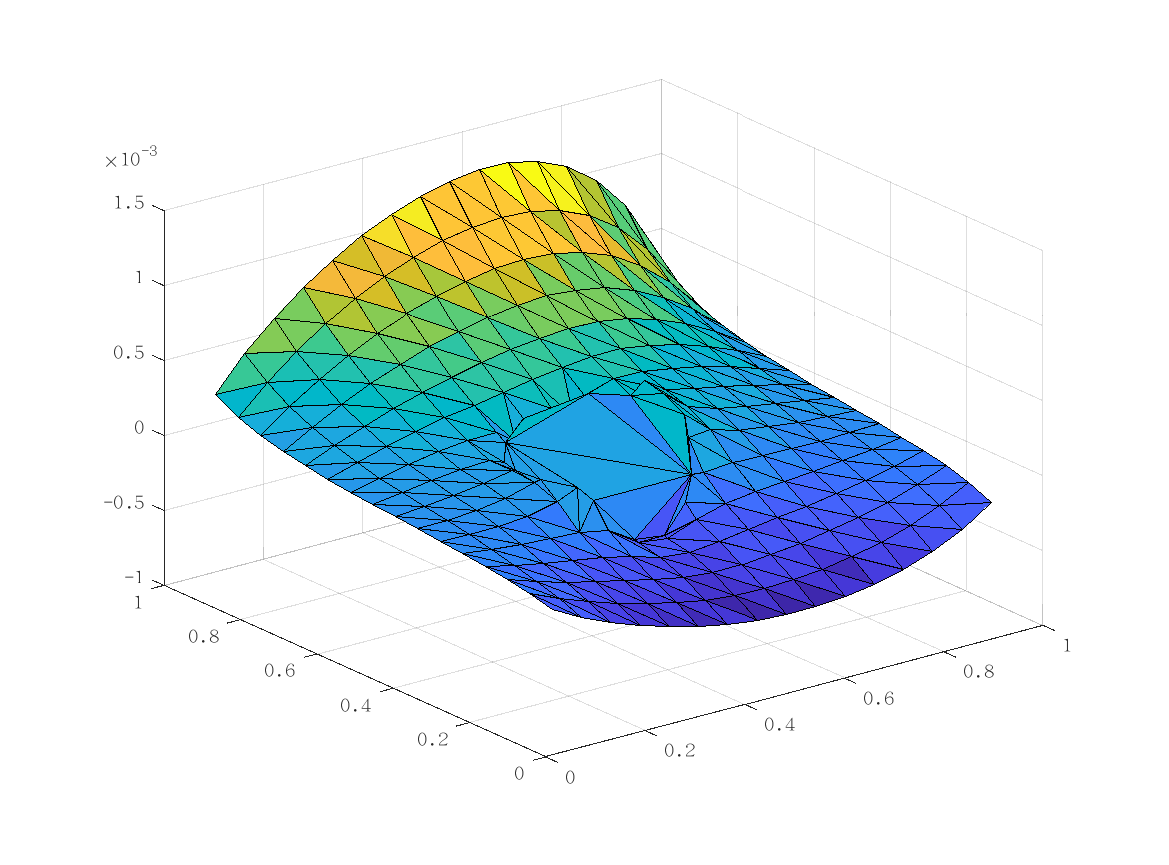
\includegraphics[width=0.95\linewidth]{figure/error_problem1_m_ir_n=16.eps}
      \caption*{$n=16$}
  \end{minipage}
  \begin{minipage}[t]{0.24\linewidth}
    \centering
    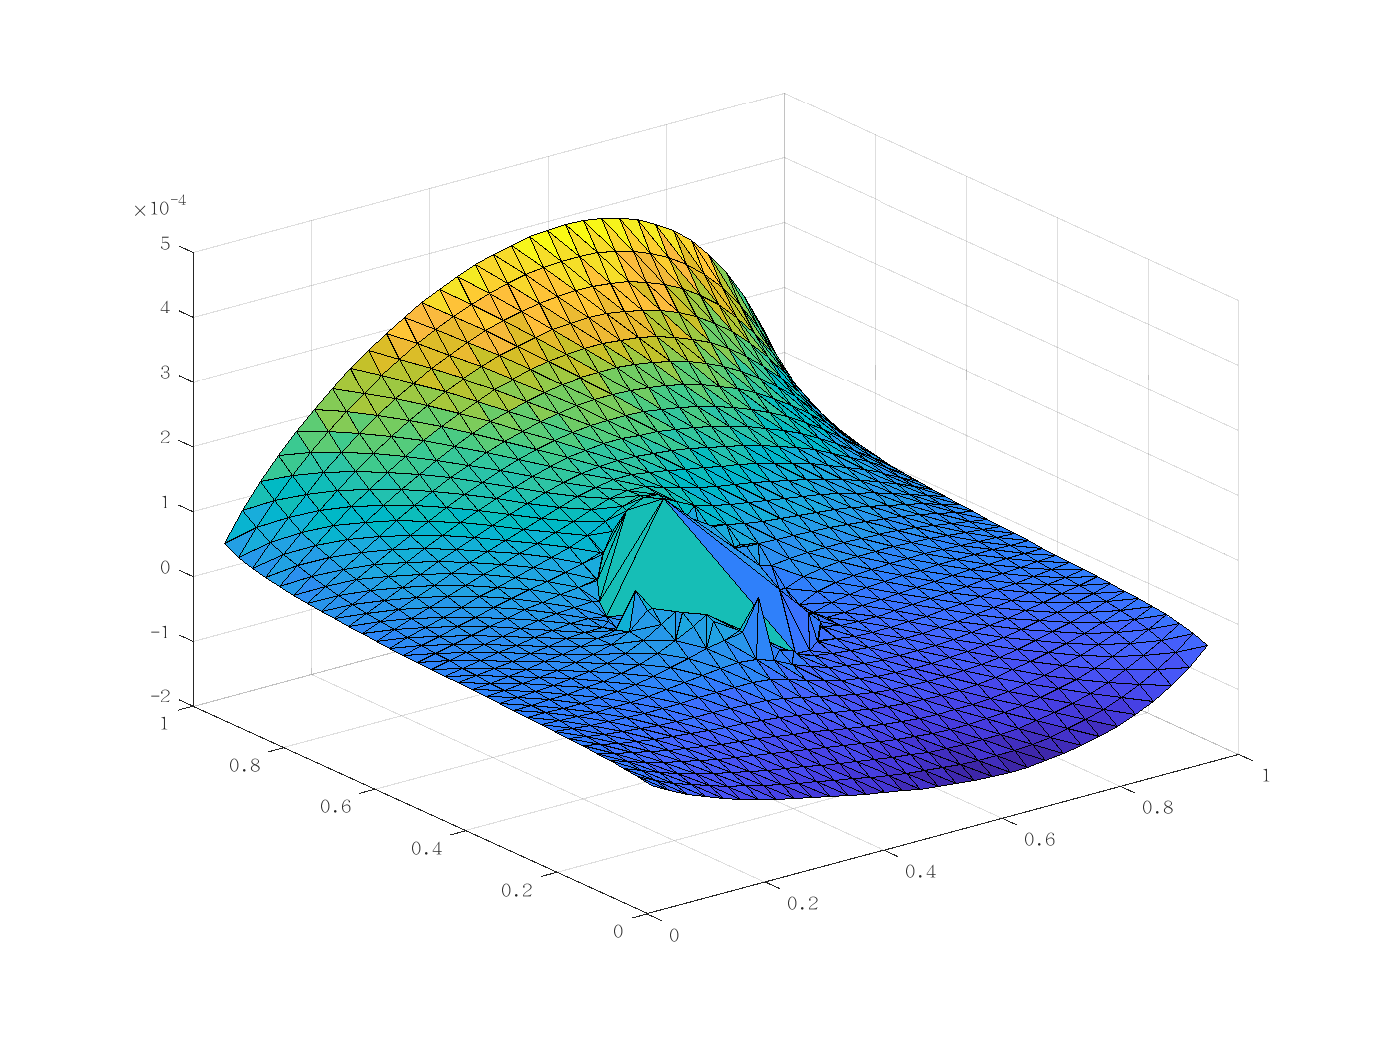
\includegraphics[width=0.95\linewidth]{figure/error_problem1_m_ir_n=32.eps}
    \caption*{$n=32$}
  \end{minipage}
  \begin{minipage}[t]{0.24\linewidth}
    \centering
    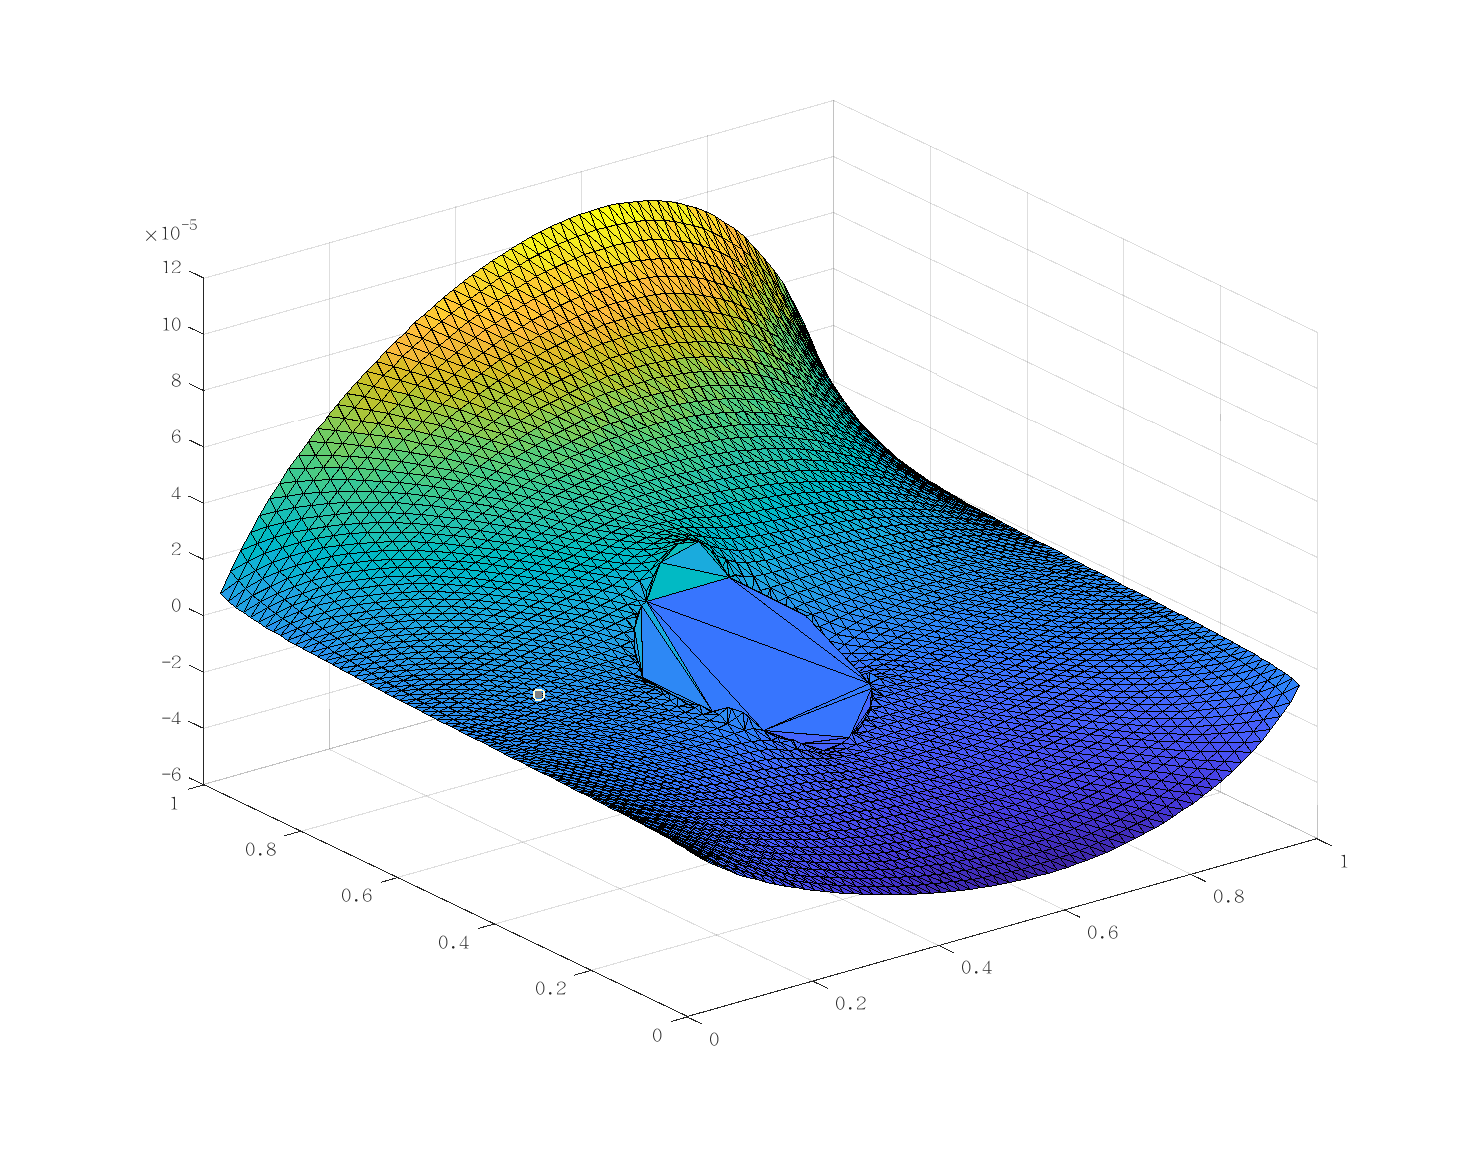
\includegraphics[width=0.95\linewidth]{figure/error_problem1_m_ir_n=64.eps}
    \caption*{$n=64$}
  \end{minipage}
  \begin{minipage}[t]{0.24\linewidth}
    \centering
    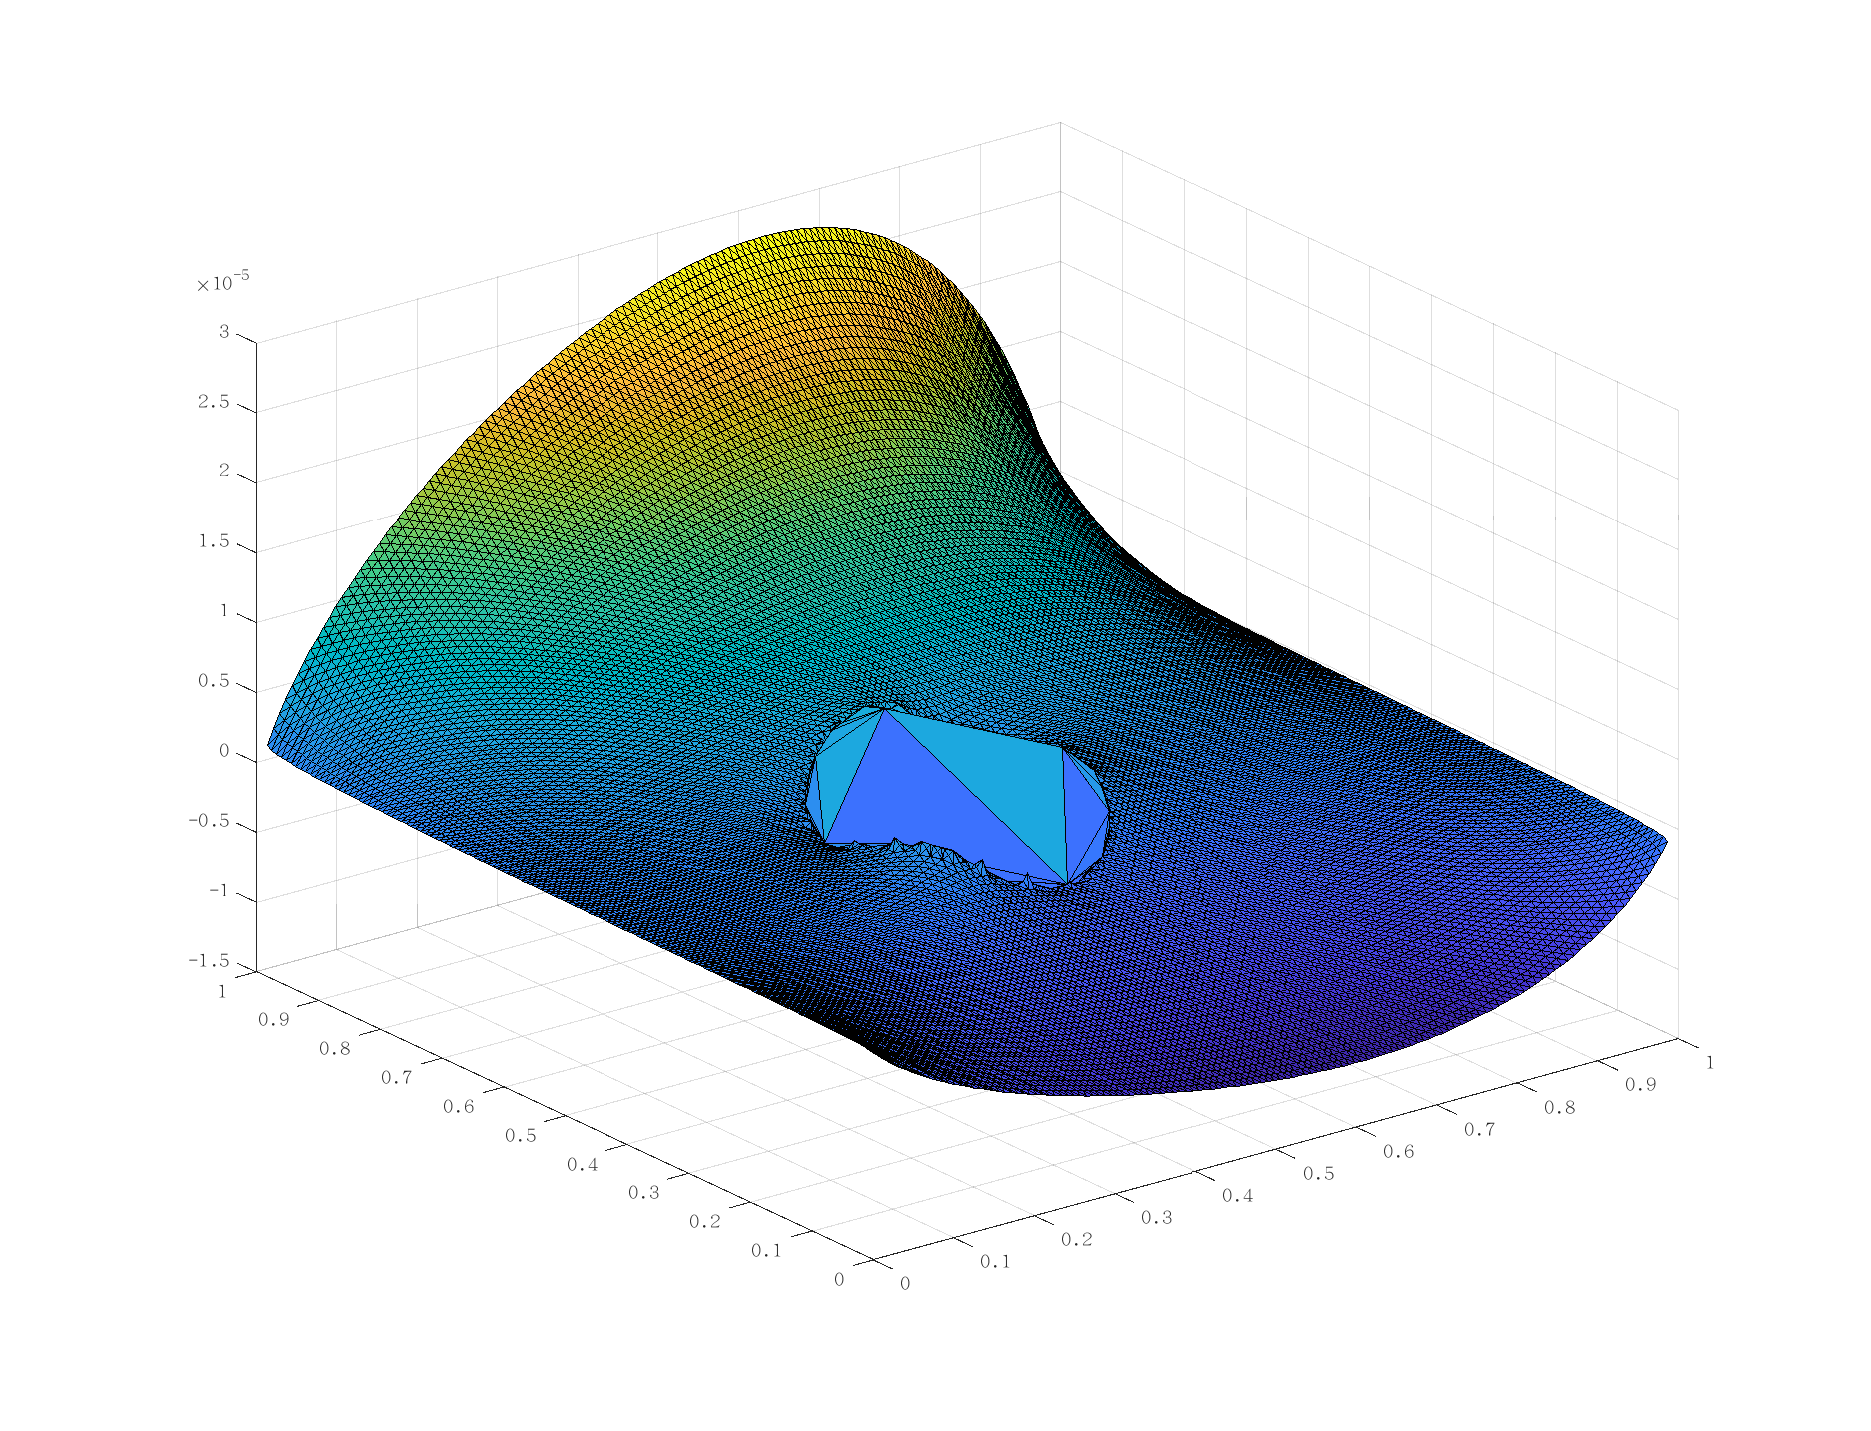
\includegraphics[width=0.95\linewidth]{figure/error_problem1_m_ir_n=128.eps}
    \caption*{$n=128$}
  \end{minipage}
\end{figure}

可以看出,越靠近Dirichlet条件下的边界,误差越小。用$1,2,\infty$范数作误差估计,如下表。

\begin{table}[H]
  \centering
  \begin{tabular}{c|cccc|c}
  \textbf{$n$}        & 16                   & 32                   & 64                   & 128                  & 收敛率 \\ \hline
  $1$-norm error      & $3.39\times 10^{-4}$ & $9.15\times 10^{-5}$ & $2.46\times 10^{-5}$ & $5.82\times 10^{-6}$ & $2.08$\\
  $2$-norm error      & $4.51\times 10^{-4}$ & $1.28\times 10^{-4}$ & $3.36\times 10^{-5}$ & $8.30\times 10^{-6}$ & $2.01$\\
  $\infty$-norm error & $1.32\times 10^{-3}$ & $4.03\times 10^{-4}$ & $1.07\times 10^{-4}$ & $2.79\times 10^{-5}$ & $1.94$
  \end{tabular}
\end{table}

再用(2)中精确解$u_2$导出相应的混合边值问题,在$x=0$与$x=1$边界上给Dirichlet条件,在$y=0,y=1$与$\partial \mathbb{D}$边界上给Neumann条件,取$\mathbb{D}=\mathbb{D}((0.45,0.45),0.15)$,用数值方法求解,得到误差与收敛率如下表。

\begin{table}[H]
  \centering
  \begin{tabular}{c|cccc|c}
  \textbf{$n$}        & 16                   & 32                   & 64                   & 128                  & 收敛率 \\ \hline
  $1$-norm error      & $6.12\times 10^{-3}$ & $1.78\times 10^{-3}$ & $4.75\times 10^{-4}$ & $1.24\times 10^{-4}$ & $1.94$\\
  $2$-norm error      & $9.71\times 10^{-3}$ & $2.92\times 10^{-3}$ & $7.91\times 10^{-4}$ & $2.08\times 10^{-4}$ & $1.93$\\
  $\infty$-norm error & $3.26\times 10^{-2}$ & $1.06\times 10^{-2}$ & $3.00\times 10^{-3}$ & $8.03\times 10^{-4}$ & $1.90$
  \end{tabular}
\end{table}

再用(3)中精确解$u_3$导出相应的混合边值问题,在$x=0,x=1$与$\partial \mathbb{D}$边界上给Dirichlet条件,在$y=0$与$y=1$边界上给Neumann条件,取$\mathbb{D}=\mathbb{D}((0.45,0.45),0.15)$,用数值方法求解,得到误差与收敛率如下表。

\begin{table}[H]
  \centering
  \begin{tabular}{c|cccc|c}
  \textbf{$n$}        & 16                   & 32                   & 64                   & 128                  & 收敛率 \\ \hline
  $1$-norm error      & $3.92\times 10^{-1}$ & $1.04\times 10^{-1}$ & $2.68\times 10^{-2}$ & $6.77\times 10^{-3}$ & $1.98$\\
  $2$-norm error      & $3.97\times 10^{-1}$ & $1.07\times 10^{-1}$ & $2.76\times 10^{-2}$ & $6.99\times 10^{-3}$ & $1.98$\\
  $\infty$-norm error & $4.48\times 10^{-1}$ & $1.22\times 10^{-1}$ & $3.18\times 10^{-2}$ & $8.09\times 10^{-3}$ & $1.97$
  \end{tabular}
\end{table}

上述三个测试函数均符合2阶收敛的理论结果。

\section{总结}

本文中所有图像均由\textbf{matlab}生成。

设计手册与测试说明见\verb|document.pdf|。

在所有的实验中,我们的求解器都取得了很好的表现,在大部分情况下,我们都验证了2阶的收敛性能。当然,对于一些较为病态的函数或条件,求解器难以准确求解方程组,从而导致了误差较大,收敛率也不准确。

值得指出的是,我们的求解器除了json文件的读取外,所有底层逻辑都是自己实现的,包括矩阵方程组的求解、数学表达式的解析等等。针对稀疏矩阵,我们对矩阵方程组的求解进行了特别优化,求解$128\times 128$的网格只需8秒。

\end{document}
